\documentclass{neu_handout}
\usepackage{url}
\usepackage{amssymb}
\usepackage{amsmath}
\usepackage{marvosym}
\usepackage{graphicx}
\usepackage[pdftex]{graphicx}
\usepackage{subfigure}
\graphicspath{ {images/} }
\everymath{\displaystyle}

% Professor/Course information
\title{Yelp Data Mining - Final Report}
\author{Emily Dutile, Vyshaal Narayanam, Xiwen Song, Yu Tian}
\date{December 2017}
\course{CS6220}{Data Mining Techniques}

\begin{document}
\section*{1 Introduction and Background}
Today we live in a society where businesses are greatly impacted by customer reviews. For some businesses, this can result in their success or failure. Looking to improve the
experience for restaurant owners and customers, we used the Yelp Open Dataset\footnote{\url{https://www.yelp.com/dataset}} that is filled with restaurant information and reviews of diverse content, along with how a customers experience was positively or negatively impacted. Through the implementation of several data mining and text mining techniques, we can better understand user reviews and gain new insights into neighborhood businesses. In this project we mine a copious amount of Yelp restaurant reviews to address the following questions: What topics are discovered frequently in reviews and do they correlate to a positive or negative review? What neighborhoods, if any, have the best selection for a particular cuisine in a certain city? Are there some areas in a city that are more upscale or divey than others? Based upon user reviews in a particular city, can we recommend a particular dish at a top restaurant?
\subsection*{1.1 The Data}
The Yelp SQL dataset contains 4.7 million reviews, 156,000 business, and 12 metropolitan areas. Spanning over 10 years of Yelp reviews and 50 states, including international countries, the dataset provides a countless number of questions to be asked. The schema\footnote{\url{https://www.yelp.com/dataset/documentation/sql}} consists of multiple tables including information about businesses, reviews, users, checkins and tips. Since we are familiar with Boston neighborhoods and its cuisines, we wanted to find a city that we thought may have some of the same characteristics. For example, the North End in Boston is known for its Italian food and South Boston is famous for it's Irish heritage and pubs. Since Boston is not in this dataset, the majority of the project focuses on restaurants in Pittsburgh, PA, due to its relatively similar characteristics. Pittsburgh has the neighborhood Bloomfield which is equivalent to our Italian North End, however, it lacks a Chinatown or Irish filled South Boston. Due to this, we were not overly confident that our clustering algorithms will be able to produce great results but they may be successful on other cities.
As seen in Figure 1, Pittsburgh is one of the leading cities with respect to its number of restaurants and has many restaurants within close proximity of one another as seen in Figure 2. The heat map of restaurants in Pittsburgh shows that a lot of the neighborhood restaurants in the center of the city are more popular.


\begin{figure}[h]
\centering
\subfigure[Number of Restaurants by City]
{
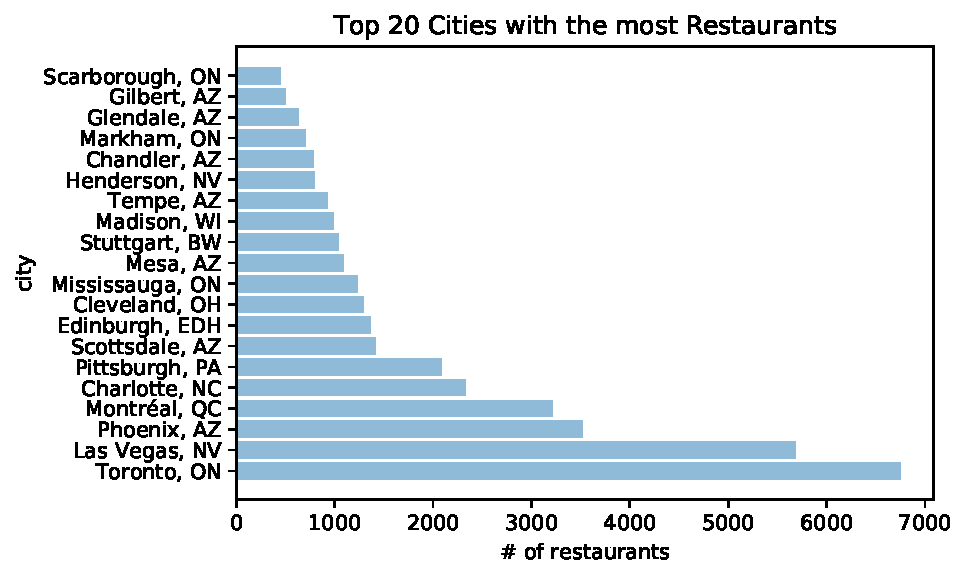
\includegraphics[width=0.47\linewidth]{cities_most_restaurants}
}
\subfigure[Heatmap of Pittsburgh restaurants]
{
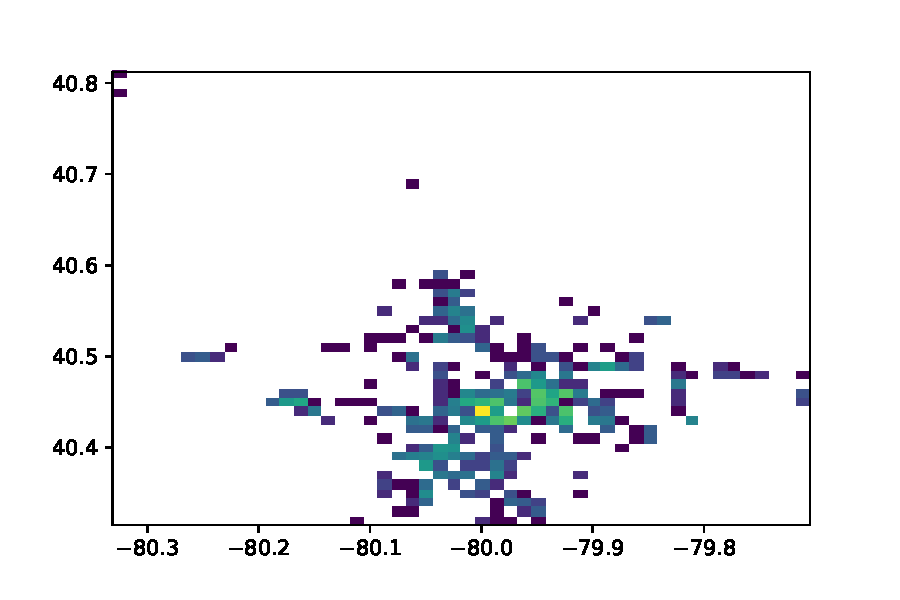
\includegraphics[width=0.45\linewidth]{pitts_heatmap}
}
\end{figure}

Pittsburgh has 2089 restaurants, 53 different neighborhoods, and a diverse cuisine selection (43 different cuisines), which made it an interesting U.S. city to us.
The team setup local databases using PyCharm and MySQLServer in order to execute faster queries. For understanding and reproducibility, the project repository and development environment set up instructions can be found on Github\footnote{\url{https://github.com/emily-jean/yelp-data-mining}}.

\subsection*{1.2 Methods}
To answer our questions, we performed data analysis and unsupervised machine learning techniques such as clustering, topic modeling and recommendation. With respect to language processing, tokenization, filtering, lemmatization, and stemming were all used for preprocessing the reviews. To tell if a customer has positive or negative feedback about a restaurant, sentimental analysis was performed in order to see if there is an interesting difference between reviews and ratings although a review is associated with a rating.

\section*{2. Exploratory Analysis}
To better visualize and explore the Pittsburgh neighborhoods a bit more, we discovered the top 10 neighborhoods with the most restaurants. Looking at other outside articles\footnote{\url{https://www.thrillist.com/eat/pittsburgh/best-neighborhoods-in-pittsburgh-for-dining-and-eating-out-ranked}}, every one of these neighborhoods are listed as one of the "Best Neighborhoods for Eating" except for Oakland. The second map on the right shows the top 10 neighborhoods with the highest average review count to give some insight as to what neighborhoods are the most popular among Yelp reviewers. In comparison to the Thrillest article, only Lawrenceville, Regent Square, Shadyside, and the Strip District are on their list.

\begin{figure}[h]
\centering
{
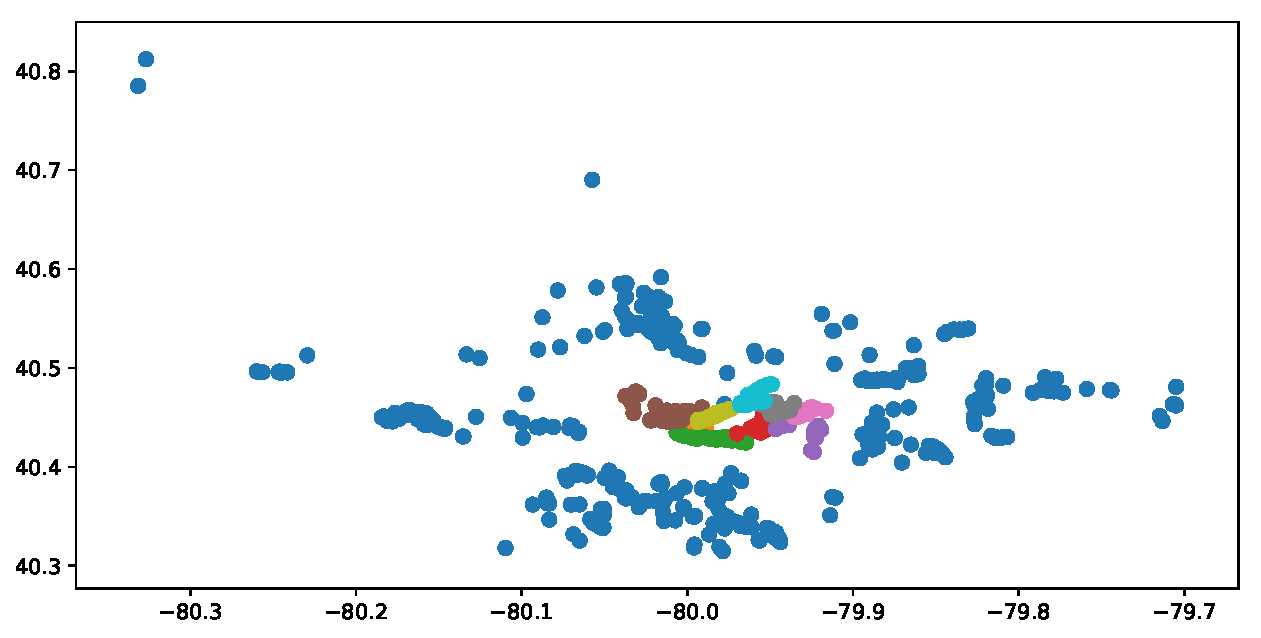
\includegraphics[width=0.4\linewidth]{top10_hoods_most_restaurants}
}
{
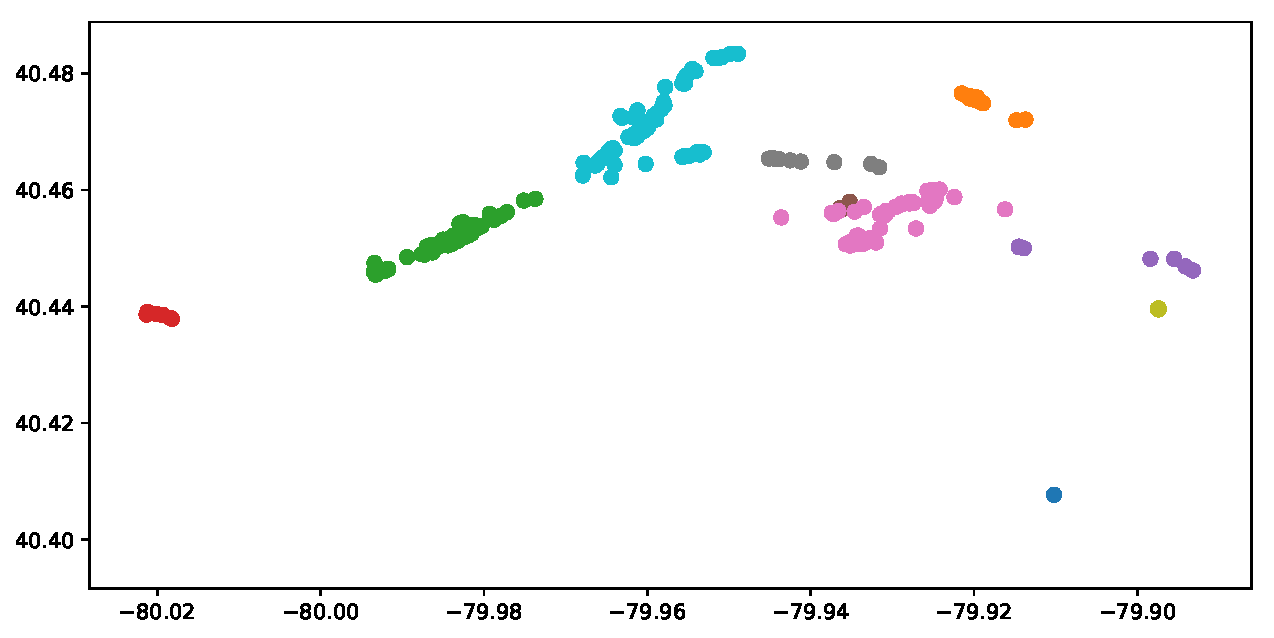
\includegraphics[width=0.4\linewidth]{top10_hoods_highest_avg_review_count}
}
{
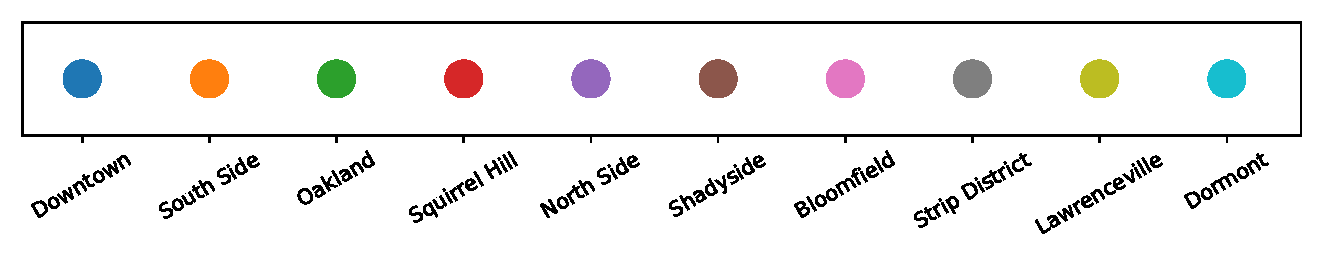
\includegraphics[width=0.4\linewidth]{legend1}
}
{
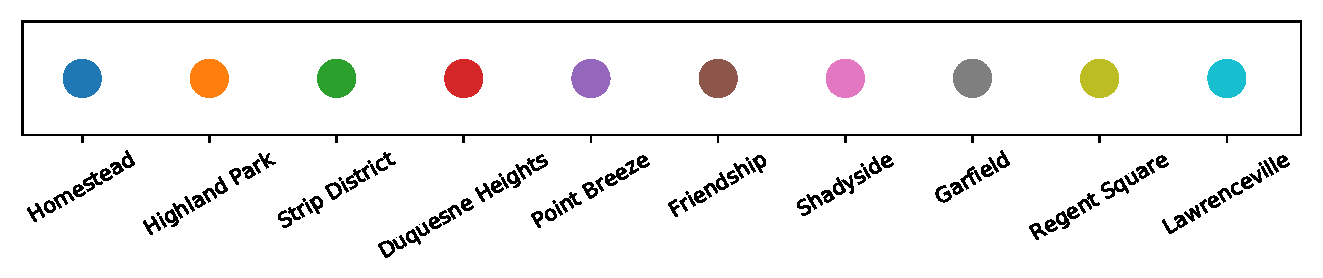
\includegraphics[width=0.4\linewidth]{legend2}
}
\caption{Pittsburgh Neighborhood Restaurants and Ratings}
\end{figure}


To get started on a deeper exploratory analysis of reviews and ratings, we plotted the distribution of the ratings for all the restaurants in Pittsburgh. From this plot we can see that most restaurants have a rating between 3 and 5. The average rating for Pittsburgh restaurants is 3.51. To gain a deeper insight of the data, we plotted the rating distribution of different cities. Although we are mostly focusing on Pittsburgh, for future analysis we would be interested in comparing differently cities to see if any interesting results arise.

\begin{figure}[h]
\centering
{
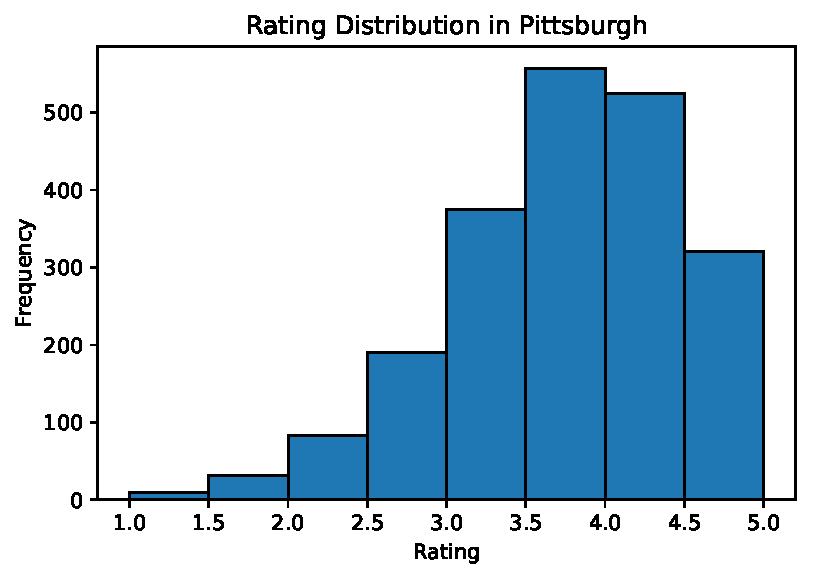
\includegraphics[width=0.3\linewidth]{rating_distribution_in_Pittsburgh}
}
{
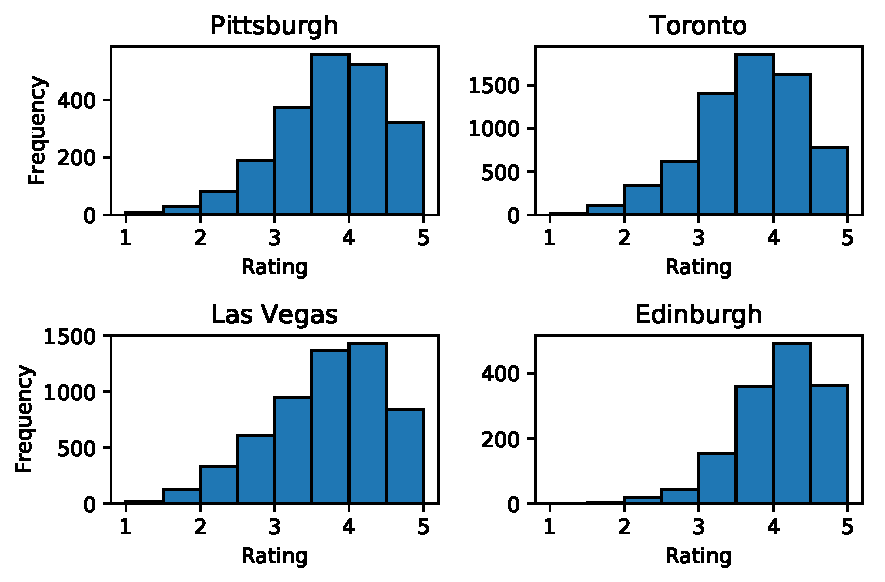
\includegraphics[width=0.3\linewidth]{rating_distribution_vs_countries}
}
\end{figure}

Besides looking at the basic distribution, we plotted the relationship between the average number of reviews and rating levels in Pittsburgh using box plot. Our original thought was that better restaurants should receive more reviews. However, the results showed us that restaurants with a medium rating acquired more reviews. After tokenization and stemming, we continued on the exploration of the relationship between average number of reviews, and the average length of review and each cuisine. We found that Japanese foods receive the most reviews while Chinese foods receive the least number of reviews in Pittsburgh. When looking at the length of review, there doesn't appear to be many differences among the variety of cuisines. 

\begin{figure}[h]
\centering
{
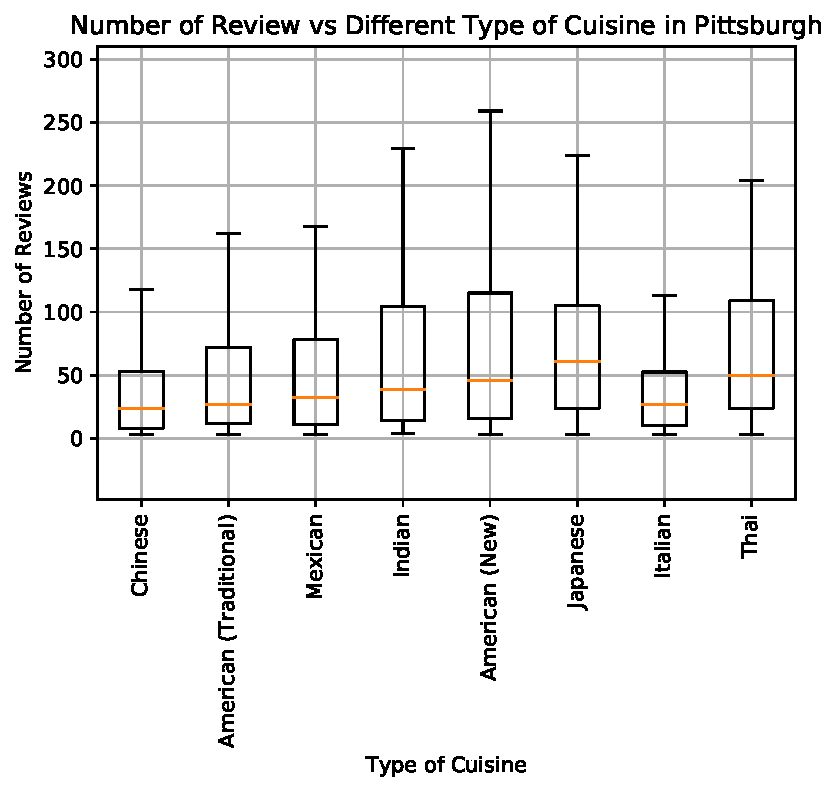
\includegraphics[width=0.35\linewidth]{number_of_review_vs_cuisine}
}
{
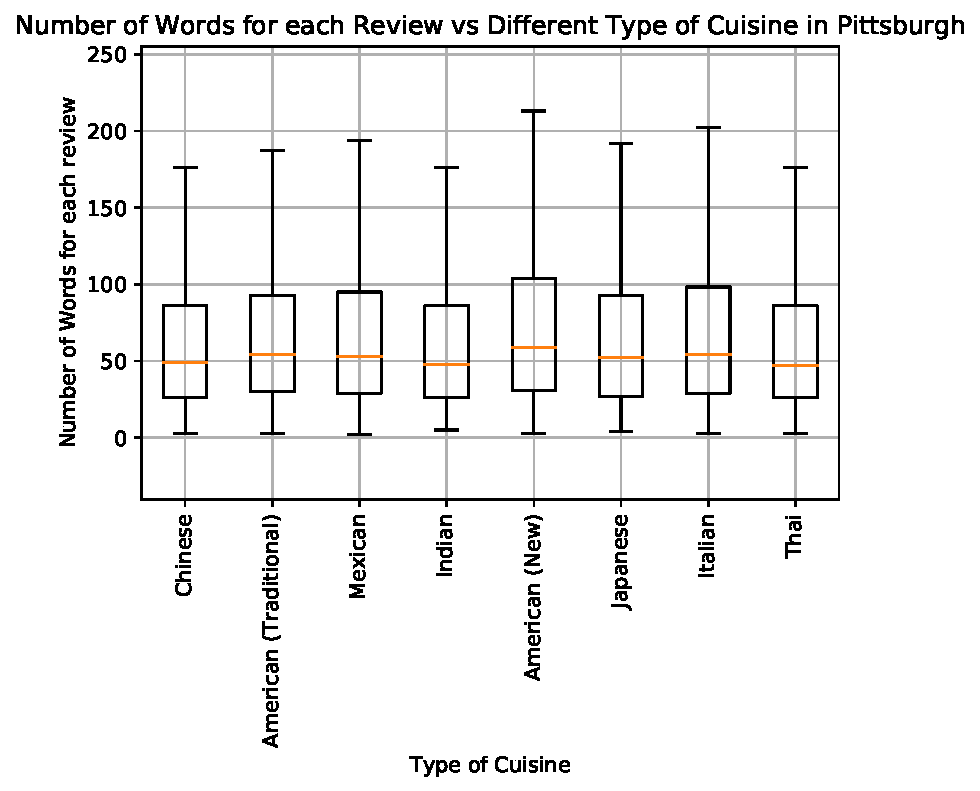
\includegraphics[width=0.4\linewidth]{average_review_length}
}
\end{figure}


Furthermore, to get a better sense on how the contents of a review correlate with the rating, we calculated the ratings for one of the restaurants by performing sentiment analysis on the reviews and then comparing the results with the dataset ratings. Through sentiment analysis, we can determine whether the review is positive or negative. We took a sample dataset of all restaurants in Pittsburgh which had more than 200 reviews to assign our own ratings (giving us 109 restaurants in Pittsburgh which satisfy our criteria), and computed the average of the values obtained from sentiment analysis of all the reviews (38,785 reviews) of that restaurant. The sentimental analysis was performed using PatternAnalyzer in NLTK (textblob is built over NLTK). We assigned a weight of +5 for a positive review and -5 for a negative review. These newly derived ratings are compared with the ratings in the original dataset as shown in the histogram. We can assume that these reviews are more accurate because we are incorporating negative weights to low star reviews.

\begin{figure}[h]
\centering
{
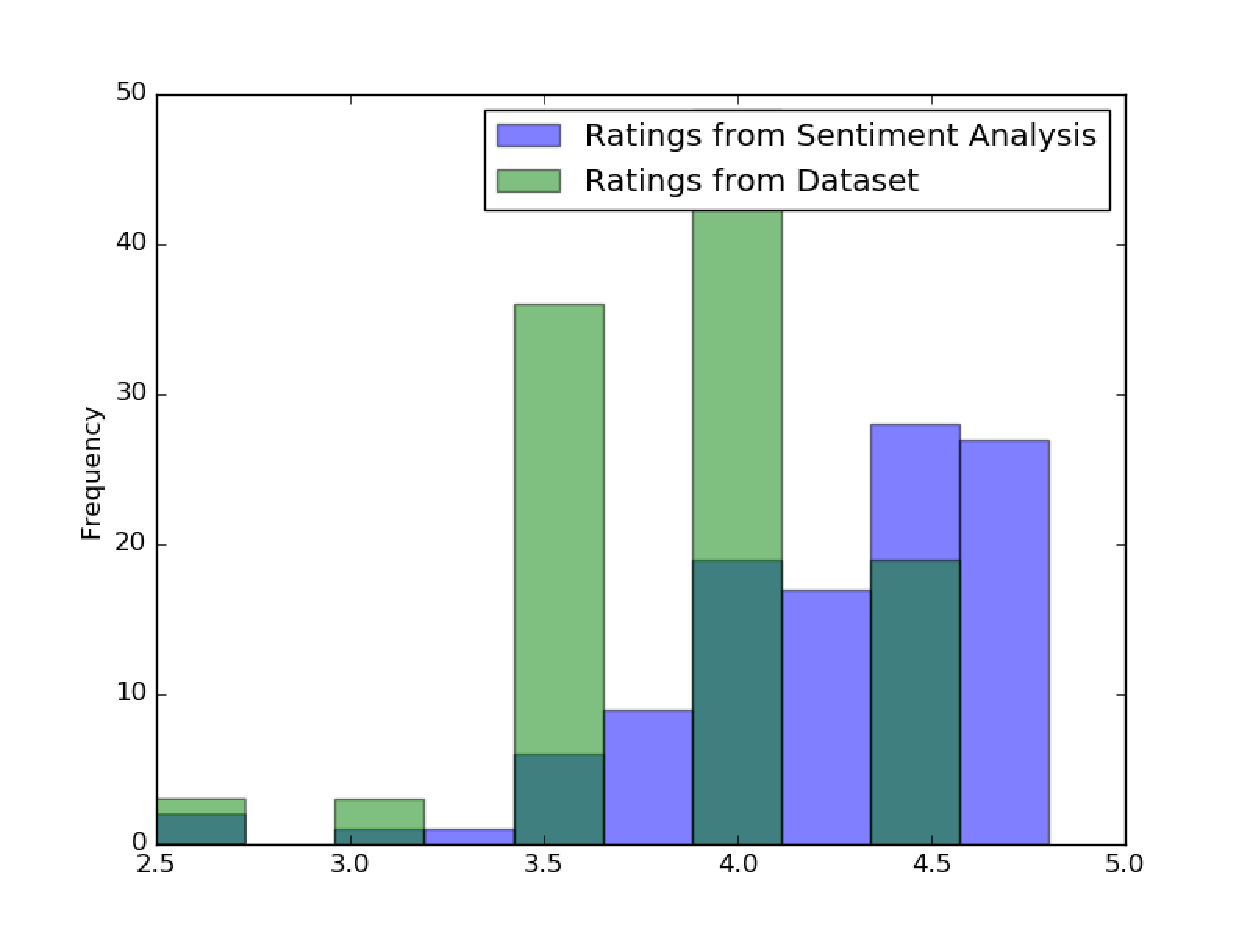
\includegraphics[width=0.4\linewidth]{sentimentanalysis}
}
\end{figure}

Next, we extracted the top 50 keywords from positive and negative reviews. Again taking a sample dataset of all restaurants in Pittsburgh that have more than 200 reviews. There are a total of 38,785 reviews. Data processing techniques such as tokenizing, filtering, stemming and filtering the key words from those reviews were performed. We then calculated 50 most frequent keywords from the negative and positive reviews separately. Negative and positive reviews were distinguished using the polarity obtained in the previous step.
The results are very promising. Few keywords such as "great","good","nice","service" came with high frequency in positive reviews where as words like "bad","good","terrible","poor","great" appeared negative reviews. Common words such as "Pittsburgh", "food", "service", and "place" are present in both positive and negative reviews. One important thing to notice is that "good" and "great" appeared in negative reviews too in a sense that customers are complaining how the food isn't that good/great. The high frequencies of words in positive reviews when compared to negative reviews is because of more number of positive reviews in the corpus.

\begin{figure}[h]
\centering
{
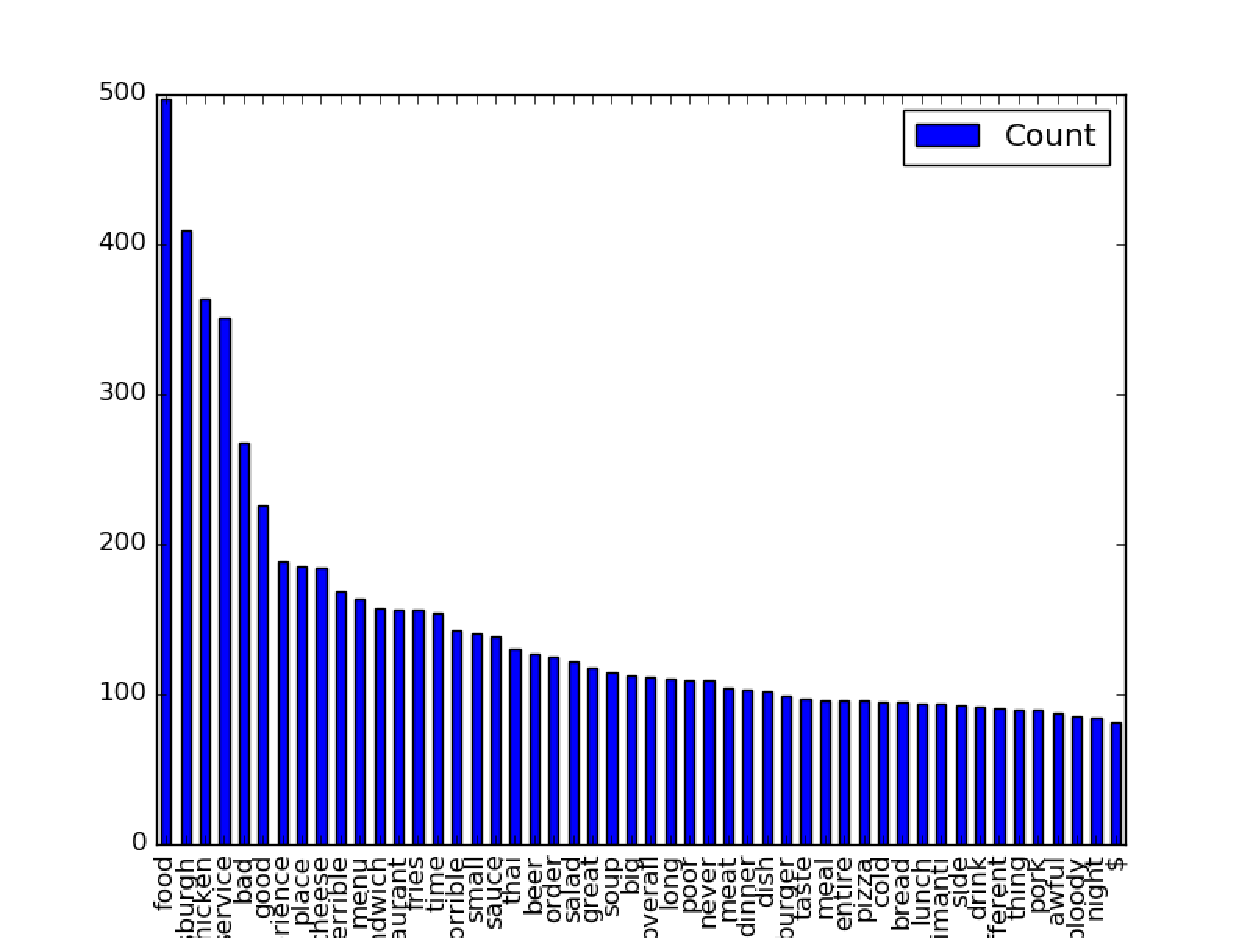
\includegraphics[width=0.4\linewidth]{top50_negativereviews}
}
{
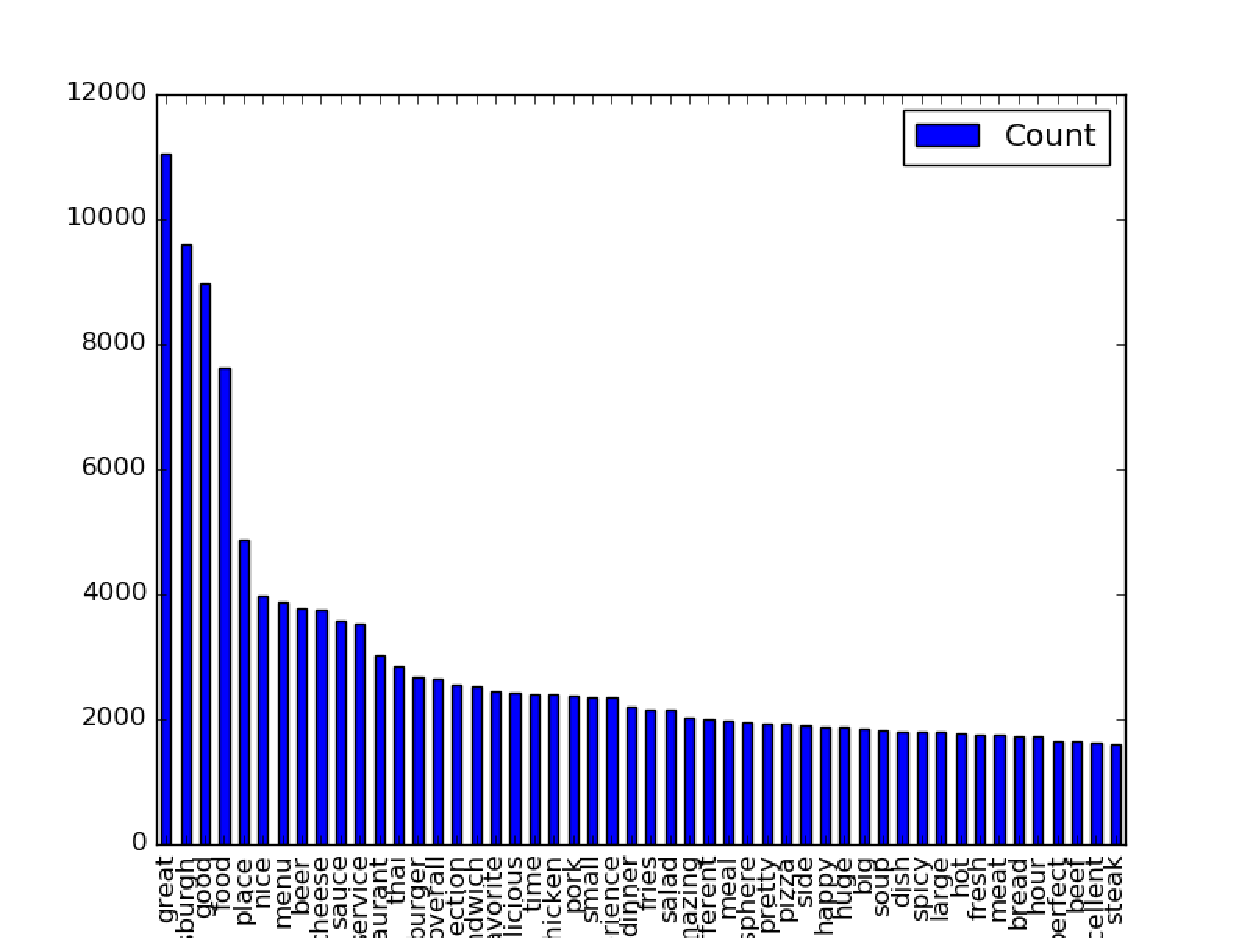
\includegraphics[width=0.4\linewidth]{top50_positivereviews}
}
\end{figure}

Although most of our exploratory analysis focused on one city, we expanded our reviews analysis to 4 different cities with the most reviews (Edinburgh, Toronto, Las Vegas, and Pittsburgh), from 3 different countries for future exploration and comparisons. The thought here was that there may be differences between different cities such as the service, or people may have different diction. It's possible that the final cluster may be verified by different external evaluation criteria, so we thought it'd be useful to further explore this area. Viewable in the Jupyter Notebook \footnote{\url{https://github.com/emily-jean/yelp-data-mining/blob/master/project/statistical_analysis.ipynb}}, we plotted the differences of rating habits among the 4 cities based on average rating score for each type of cuisine. Edinburgh has the best rating feedback, relatively speaking, while Toronto seems to be lacking Yelper feedback.


\section*{3 Data Mining Analysis}

\subsection*{3.1 Geographic Based Clustering}
To find what cuisines may lie in particular neighborhoods in Pittsburgh, we performed three different clustering techniques: K-Means, GMM and DBSCAN. K-Means and GMM seemed to provide the best clustering results so these methods were more heavily used and evaluated.

\begin{figure}[h]
\centering
\subfigure[All Restaurants in Pittsburgh]
{
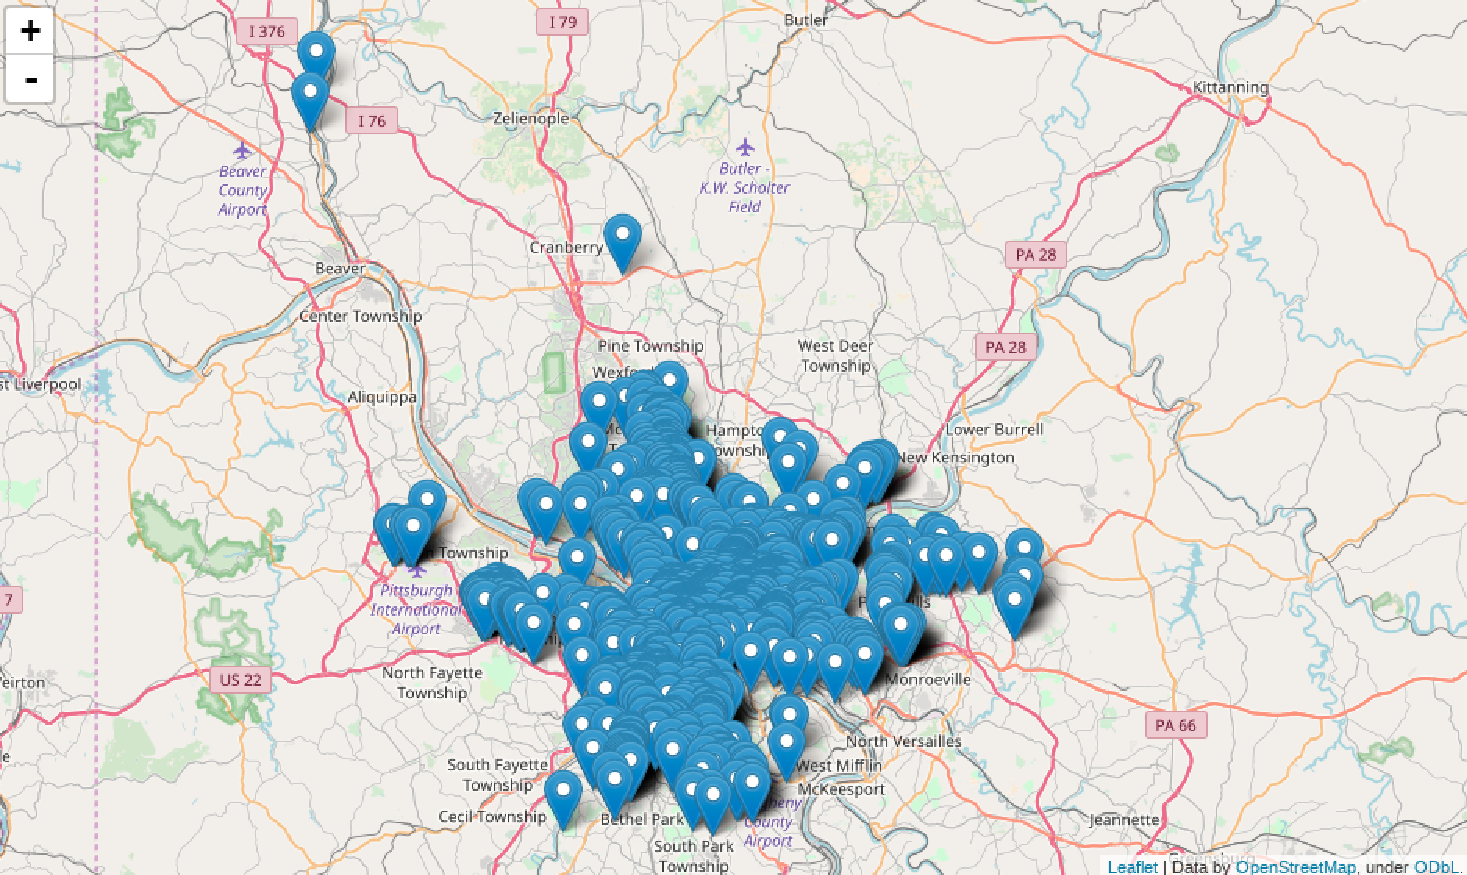
\includegraphics[width=0.35\linewidth]{all_restaurants_pitts}
}
\subfigure[Pittsburgh Neighborhoods with the most restaurants]
{
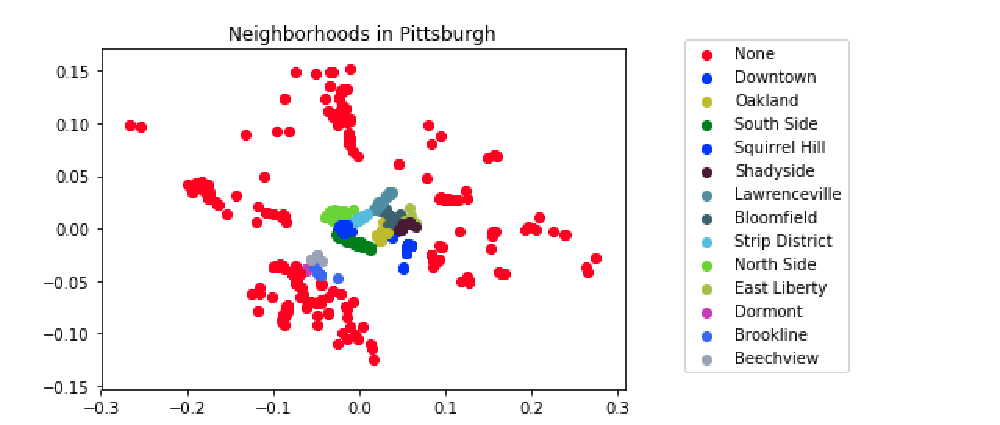
\includegraphics[width=0.55\linewidth]{pittsburgh_hoods}
}
\end{figure}

In order to run these algorithms, we decided to look at the closeness and similarities of the restaurants by using the longitude and latitude which considered cluster closeness, as well as the category/cuisines to cluster for similarity. During the data exploration, we dug into all the types of categories, realizing that we would want to filter out other non-restaurant businesses as well as things such as 'cafe' or 'breakfast' which we didn't identify as a cuisine. This left us with a list of 49 cuisines. We didn't consider any cuisine that had less than 10 restaurants and we also ended up excluding restaurants that weren't tagged within a neighborhood. As seen back in Figure 1, there were a significant amount of restaurants that didn't fall within a neighborhood according to the dataset. After running K-Means a few times, we found more reasonable results by also excluding neighborhoods that had less than roughly 8 restaurants based upon these cuisines and those that didn't have a neighborhood tag.
\\\\
The SQL data was parsed into a pandas dataframe which has two columns for latitude and longitude, and the remaining are all the cuisines in Pittsburgh. Using the one-hot method, if a restaurant is of that cuisine then the value for the column is 1. To account for the curvature of the earth, though you might want to adjust degrees of longitude and latitude, feature scaling was performed on longitude and latitude in order to scale down the location to a range of cuisines. This was done by subtracting the mean of the whole column from each value, dividing that by the standard deviation in order to get the z-score. As seen below, we selected 4 to be the appropriate number of clusters for KMeans++ by creating a plot to show the error vs. the number of clusters since it appears to be the greater 'bend' in the elbow. As shown in the figures below, the longitude/latitude of the restaurants have been plotted and each cluster is labeled with a cuisine.

\begin{figure}[h]
\centering
{
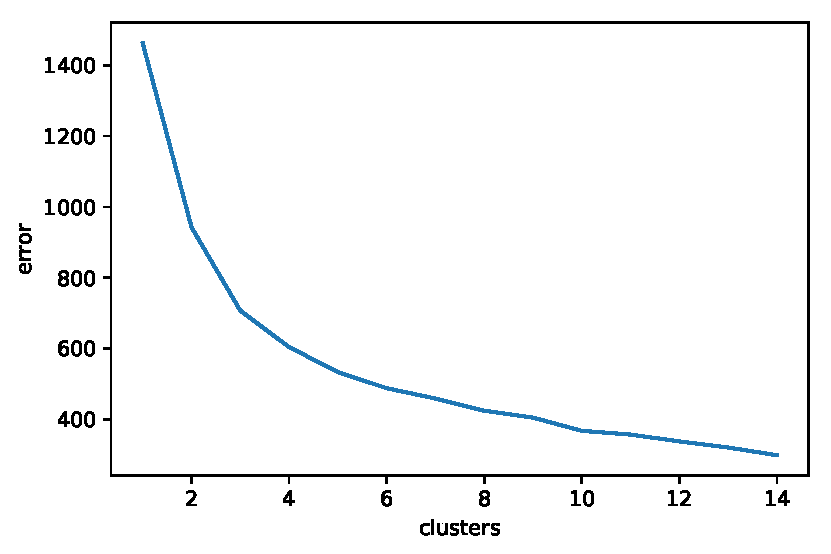
\includegraphics[width=0.35\linewidth]{kmeans_error}
}
{
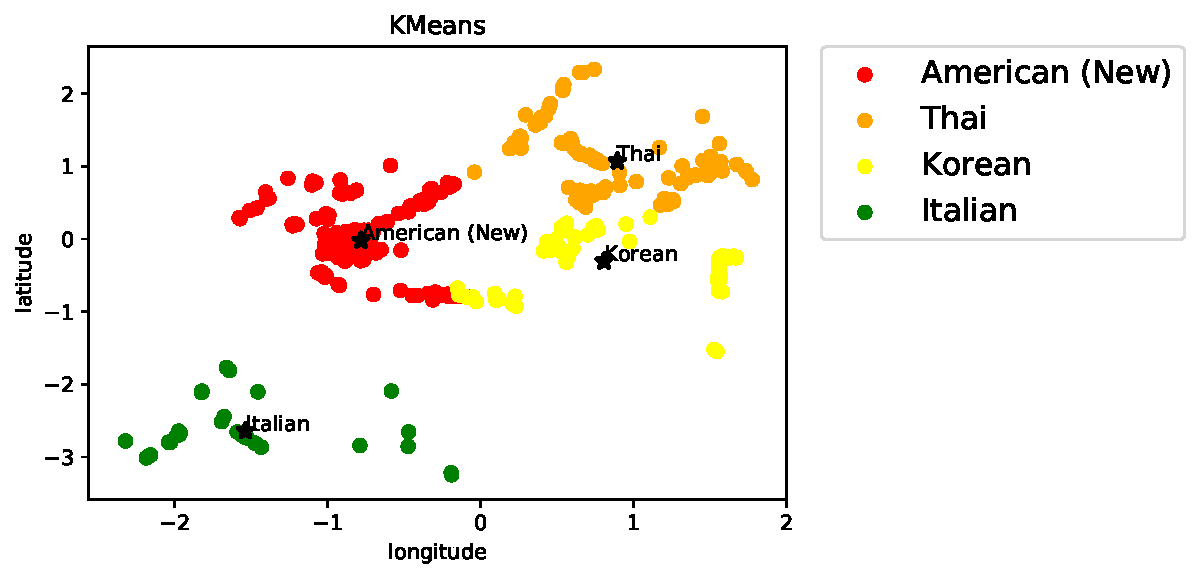
\includegraphics[width=0.5\linewidth]{kmeans_cuisines}
}
\end{figure}


In order to avoid dominance of a particular cuisine purely because the number of restaurants it has in Pittsburgh, the ratio of each cuisine in the cluster with the total number of restaurants in that category was calculated. From this, the category that has the maximum ratio was selected to be the cluster label. With our original intention to cluster cuisines by neighborhoods, K-Means has a more well-defined clusters since each point only belongs to one cluster. On the other hand, GMM had over-lapping clusters since it calculates the probability of a point belonging to each cluster and therefore seemed to give better clustering. The two results visually had similar clustering. When increasing n components to 15 in the gaussian mixture model, the silhouette score slightly increased to 0.31. The results can be found in the appendix.\\

When running K-Means on this dataset, we received a silhouette score of 0.29. This indicates that there doesn't seem to be many neighborhoods or districts within Pittsburgh that seem to be overly known for a specific cuisine. Bloomfield is known as Pittsburgh's "Little Italy", which was expected to be seen in the upper right, and it has been said that Squirrel Hill is Pittsburgh's Korean neighborhood. Pittsburgh doesn't seem to have as many neighborhoods that are divided by cuisine or culture, so these results may make some sense. K-Means was also run with the latitude and longitude only to see how it handled clustering the neighborhoods. Visually, it looked fairly close to what the true neighborhood tags are, and we received a silhouette score of 0.61. K-Means was also run within specific neighborhoods, Downtown and Bloomfield were both tried. Unfortunately, the score did not increase drastically for any neighborhood and no overly interesting results were found.

\begin{figure}[h]
\centering
{
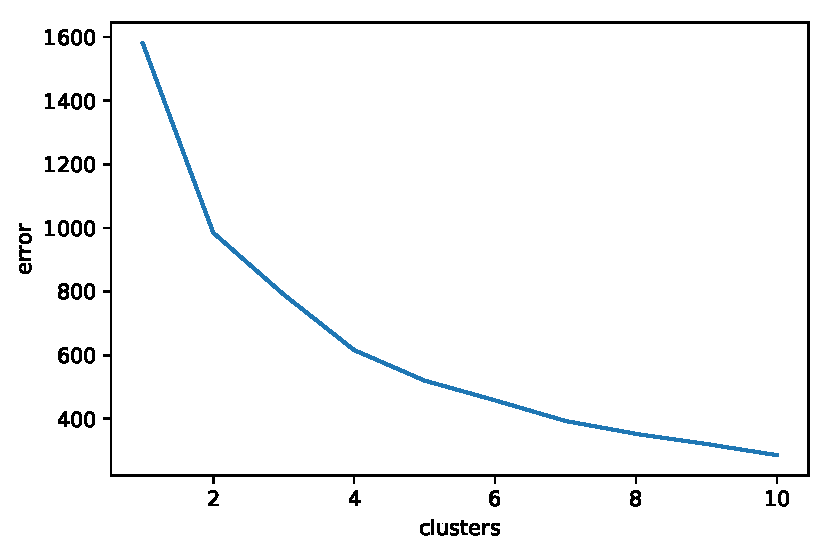
\includegraphics[width=0.38\linewidth]{error_kmeans_attributes}
}
{
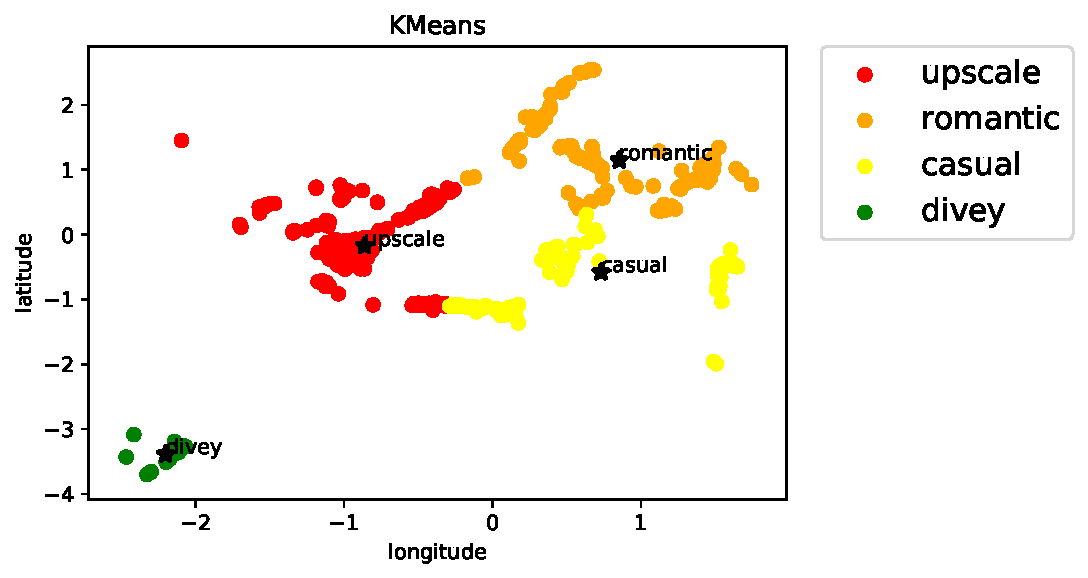
\includegraphics[width=0.5\linewidth]{kmeans_attributes}
}
\end{figure}


To find out if there are areas in the city that have a particular attribute, we took restaurants into consideration that had attributes of either upscale, divey, classy, casual, touristy, trendy or romantic. Again, we filtered out the neighborhoods that had less than 10 restaurants, which left us with over 630 restaurants. As seen above in the two images above, we found that the best number of clusters to select was 4. This time, we received a higher silhouette score of .38 which was more promising. Seeing that the downtown area was determined to have a label of upscale seemed very appropriate. In comparison to an interactive map of Pittsburgh\footnote{\url{http://www.city-data.com/nbmaps/neigh-Pittsburgh-Pennsylvania.html}}, these labels seemed to be somewhat accurate with respect to the house-hold income by neighborhood. With more time, we would have liked to explore this area more.




\subsection*{3.2 Review-based Recommendation System}
Review analysis is very useful under many recommendation system scenarios. For our project, we built a recommendation system based on the reviews of each restaurant. Restaurant profiles and user profiles were built up based upon the text review information. To transfer the words vectors to numeric vectors, TF-IDF method was used. By matching users’ review profile with the most similar cluster of restaurants, a simplified review based recommendation system was developed.

\subsubsection*{3.2.1 TF-IDF}
\textbf{TF-IDF} stands for term frequency–inverse document frequency, which is a numerical statistic that is intended to reflect how important a word is to a document in a corpus. TF-IDF was used to turn text data into a numeric vector. The method is an extension of the frequent itemset concept. The \textbf{TF} which stands for term frequency, is the number of times a term occurs in a document. The more frequent a word appears in one document, the more important this term is for a certain document. \textbf{IDF} stands for the inverse document frequency, which diminishes the weight of terms that occur very frequently in the document set and increases the weight of terms that occur rarely. The TF-IDF weight is the product of the TF term and the IDF term. Terms with higher TF-IDF scores are better to represent the information of each document and vice versa.

\subsubsection*{3.2.2 Text Review to Numeric Matrix and Clustering}
All the restaurants and reviews of restaurants in Pittsburgh were extracted from the yelp SQL dataset, and the reviews for each restaurant were merged into a single document. By using the NLTK package, we preprocessed the raw text review data through tokenization, stemming and lemmatization. Next, a dictionary was built up containing all the preprocessed words. The team implemented our own TF-IDF algorithm and turned the text review profile into a numeric TF-IDF weight profile for each restaurant. K-means clustering algorithm was then run using the K-means ++ method offered by the sklearn package. The relationship between the cluster number and SSE is shown in the graph below. In this case, SSE does not look to be a very good criteria to determine K since there is not an obvious "elbow" in the graph. Ideally, other methods would be used to pick an appropriate number of clusters. 

\begin{figure}[h]
\centering
{
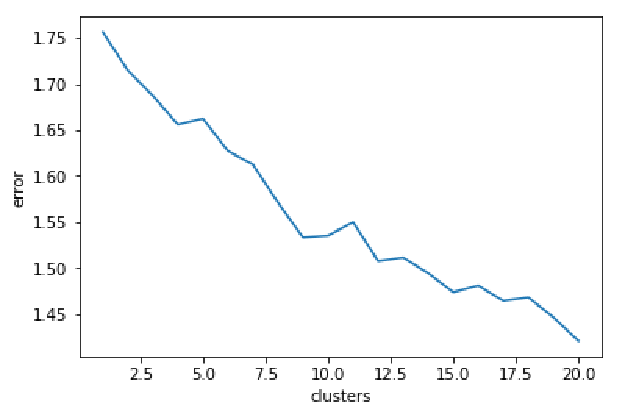
\includegraphics[width=0.4\linewidth]{KvsError}
}
\caption{Relationship between K and Error}
\end{figure}

\subsubsection*{3.2.3 Evaluation for Recommendation System Performance}
We picked several sample users to build up the users’ review profile. We implemented a user based recommendation system to find out the most similar cluster to the user profiles. To evaluate the results, we checked the average rating score of the restaurants a user has been to in the clusters. The reviewed analysis improves the performance of recommendation system if the score is above the average score of all restaurants in the cluster and all restaurants the user has been. 
 
\subsection*{3.3 Topic Modeling}

Topic modeling is a text-mining tool for discovery of hidden semantic structures in a text body. This is an unsupervised learning technique that assumes documents are produced from a mixture of topics. The "topics" produced by topic modeling techniques are clusters of similar words. Using contextual clues, topic models can connect words with similar meanings and distinguish between uses of words with multiple meanings. 
The most common topic models are Latent Semantic Indexing (LSI), Latent Dirichlet Allocation (LDA), Hierarchical Dirichlet Process (HDP). The main idea of all these models is to find the "abstract" topics that occur in a collection of documents. We chose to use LDA since it is the most preferred due to it results by using a generative probabilistic model.

\subsubsection*{3.3.1 Latent Dirichlet Allocation}
Latent Dirichlet allocation (LDA) is a particularly popular method for fitting a topic model. It models each document as a dirichlet mixture of topics, and each topic as a mixture of words. This allows documents to overlap with each other in terms of content, rather than being separated into discrete groups.\\

We filtered the dataset down to restaurants in Pittsburgh that have atleast 200 reviews (there are 109 restaurants and 38,785 reviews that match our criteria). This allowed us to extract the latent subtopics and pinpoint areas of interest. We distinguish these reviews as positive reviews and negative reviews based on their rating. To reduce noise, data cleaning of these reviews was performed. Only terms that occur atleast 10 times in the corpus were included into the training model because the less frequent terms wouldn't be contributing much to the topic and they increase the size of the document vector. This leads to more training time as well. We used gensim, a tool for discovering the semantic structure of documents by examining the patterns of words. The cleaned reviews were fed to LDA model, and below are word clouds of 8 topics consisting of different words. Note that the same word can be present in multiple topics. Also note that we can get any number of topics we want. We set it to 8 in order to get a brief overview of what the data looks like. The font size in the word cloud indicates the frequency of the word in the topic. The higher the frequency of the word in topic, the higher would be the font.

\begin{figure}[h]
\centering
{
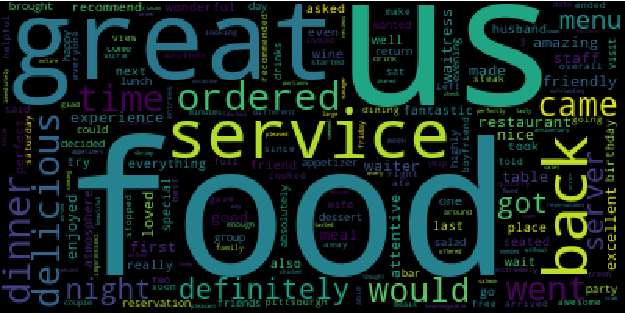
\includegraphics[width=0.2\linewidth]{lda_positive_1}
}
{
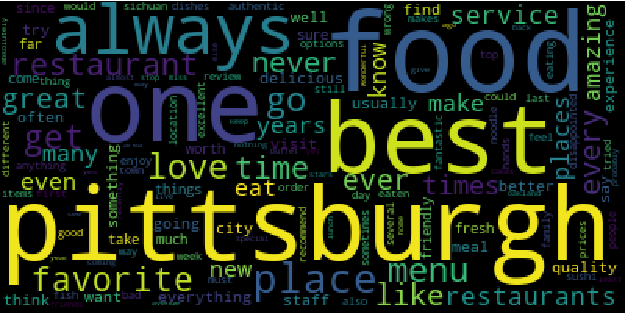
\includegraphics[width=0.2\linewidth]{lda_positive_2}
\vspace{0.1cm}
}
{
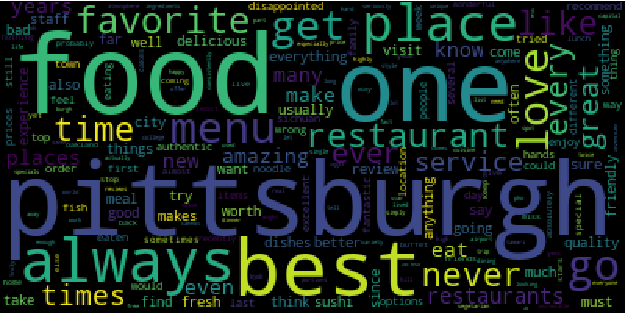
\includegraphics[width=0.2\linewidth]{lda_positive_3}
}
{
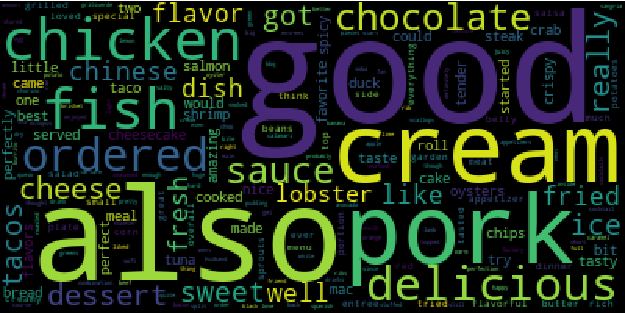
\includegraphics[width=0.2\linewidth]{lda_positive_4}
\vspace{0.1cm}
}
{
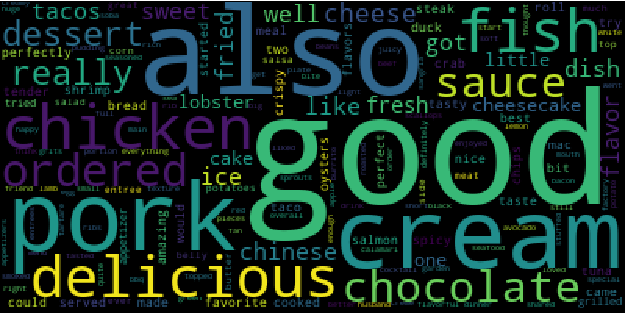
\includegraphics[width=0.2\linewidth]{lda_positive_5}
}
{
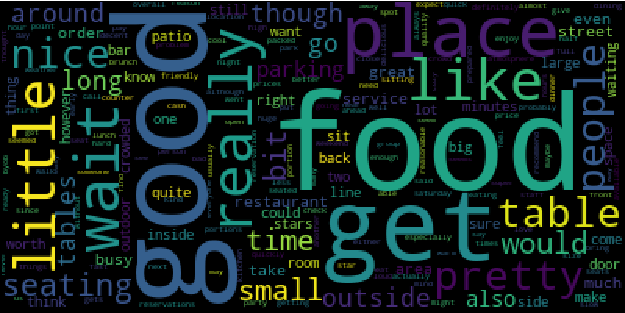
\includegraphics[width=0.2\linewidth]{lda_positive_6}
\vspace{0.1cm}
}
{
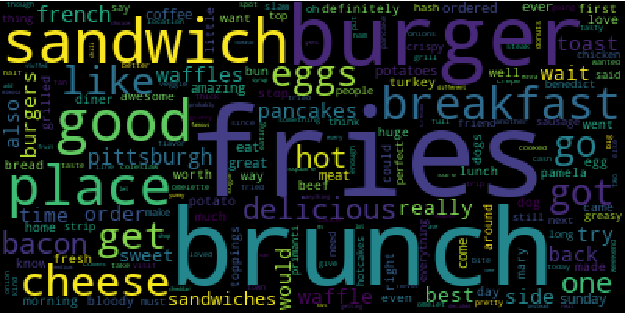
\includegraphics[width=0.2\linewidth]{lda_positive_7}
}
{
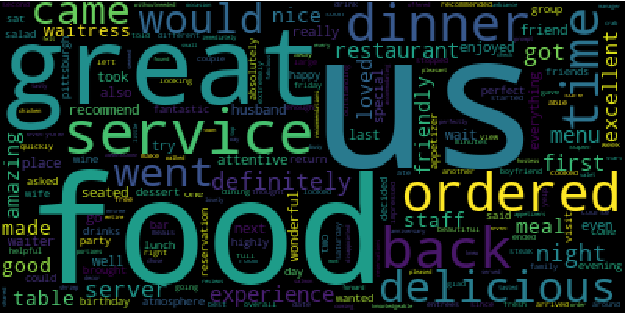
\includegraphics[width=0.2\linewidth]{lda_positive_8}
}
\caption{LDA Positive Results using WordClouds}
\end{figure}


\begin{figure}[h]
\centering
{
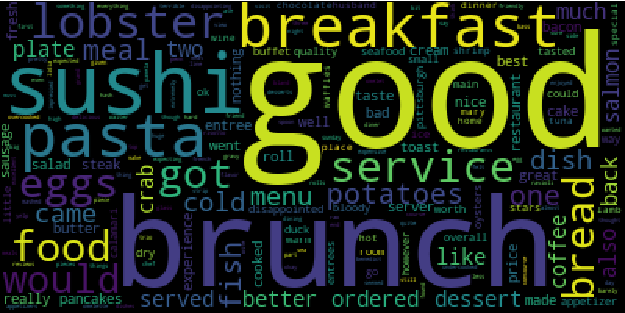
\includegraphics[width=0.2\linewidth]{lda_negative_1}
}
{
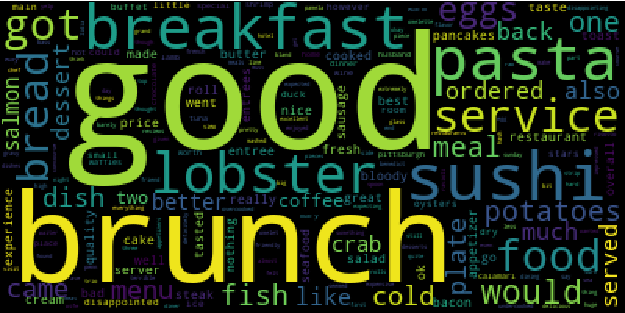
\includegraphics[width=0.2\linewidth]{lda_negative_2}
\vspace{0.1cm}
}
{
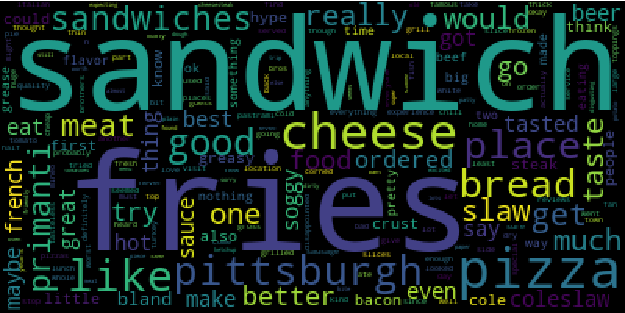
\includegraphics[width=0.2\linewidth]{lda_negative_3}
}
{
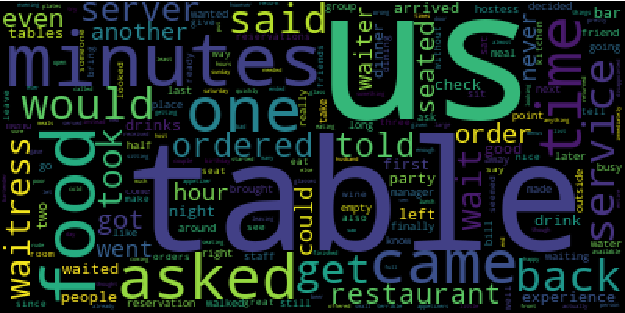
\includegraphics[width=0.2\linewidth]{lda_negative_4}
\vspace{0.1cm}
}
{
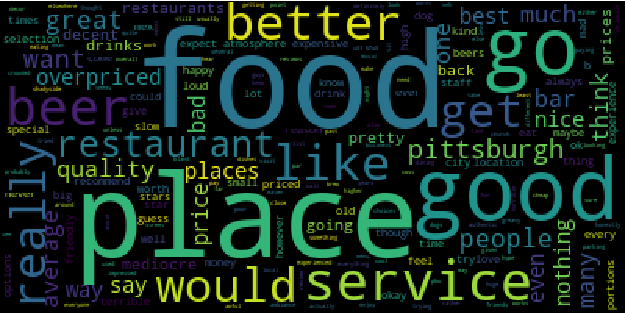
\includegraphics[width=0.2\linewidth]{lda_negative_5}
}
{
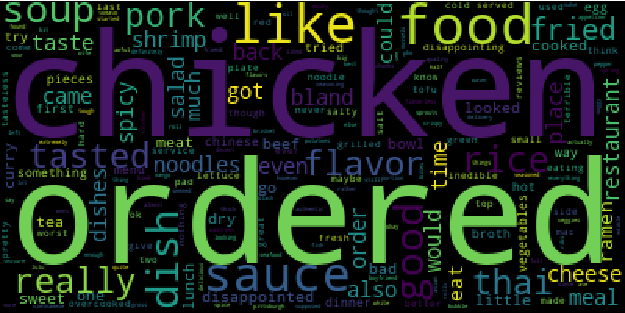
\includegraphics[width=0.2\linewidth]{lda_negative_6}
\vspace{0.1cm}
}
{
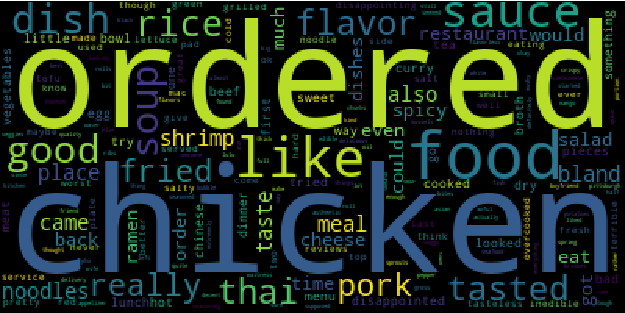
\includegraphics[width=0.2\linewidth]{lda_negative_7}
}
{
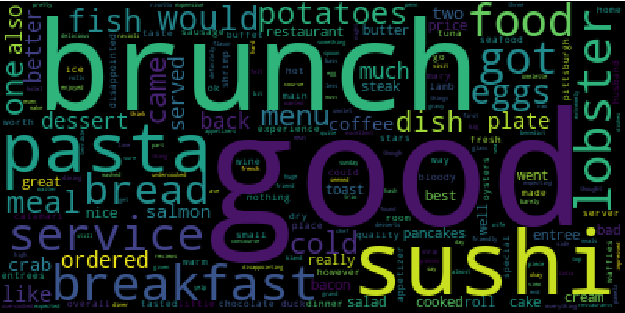
\includegraphics[width=0.2\linewidth]{lda_negative_8}
}
\caption{LDA Negative Results using WordClouds}
\end{figure}

Orginally, we observed that words like “place”, “good”, ”food”, and ”chicken” were found in almost all the word clouds because we had selected a poor number of topics. This was improved by training the model with a greater number of latent features (number of topics). With a very high number of topics, we needed a better tool for exploratory analysis.\\

ADD VYSHAAL'S UPDATE HERE.\\

The high font size of words like “place”, ”good”, and ”food” in all the word clouds is due to the very high frequency of these words in their respective topics. If we increase the number of topics, repetition of these words in multiple wordclouds would decrease but the font size in their respective word cloud would not decrease. 

\subsubsection*{3.3.2 Visualization using PyLDAVis}
pyldavis, a Python LDA Visualization tool for LDA Models was used to create visuals for our LDA model. In A.2 of the Appendix, a visual for the LDA model on negative reviews with 50 topics can be found. For a more detailed exploratory analysis, download this\footnote{\url{https://github.com/emily-jean/yelp-data-mining/blob/master/project/topic-modeling/visualization_negative_50.html}} html page and run it in your browser.\\

In LDA model on negative reviews we have 50 circles representing each topic. The area of a circle represents the prevalence of the topic. The length of the bars on the right represent the membership of a term in a particular topic. In addition to visualizing topic prevalence, the left pane shows inter-topic differences. The distance between topics is calculated using Jenson Shannon Distance, a method of measuring similarity between two probabilistic distributions. A topic in LDA is a multinomial distribution over the (typically thousands of) terms in the vocabulary of the corpus. It can also be inferred that topics consisting of the same/similar words are close to each other. Each topic’s overall prevalence is encoded using the areas of the circles, where topics are sorted in decreasing order of prevalence. Note the Area of topic 1 $>$ topic 2 $>$ ... Topic50. When topic 1 is clicked, the right panel of the visualization depicts a horizontal barchart whose bars represent the individual terms that are the most useful for interpreting the currently selected topic on the left. Words with high frequency are present in the top of the panel. A pair of overlaid bars in the right panel represent both the corpus-wide frequency of a given term as well as the topic-specific frequency.

\begin{figure}[h]
\centering
{
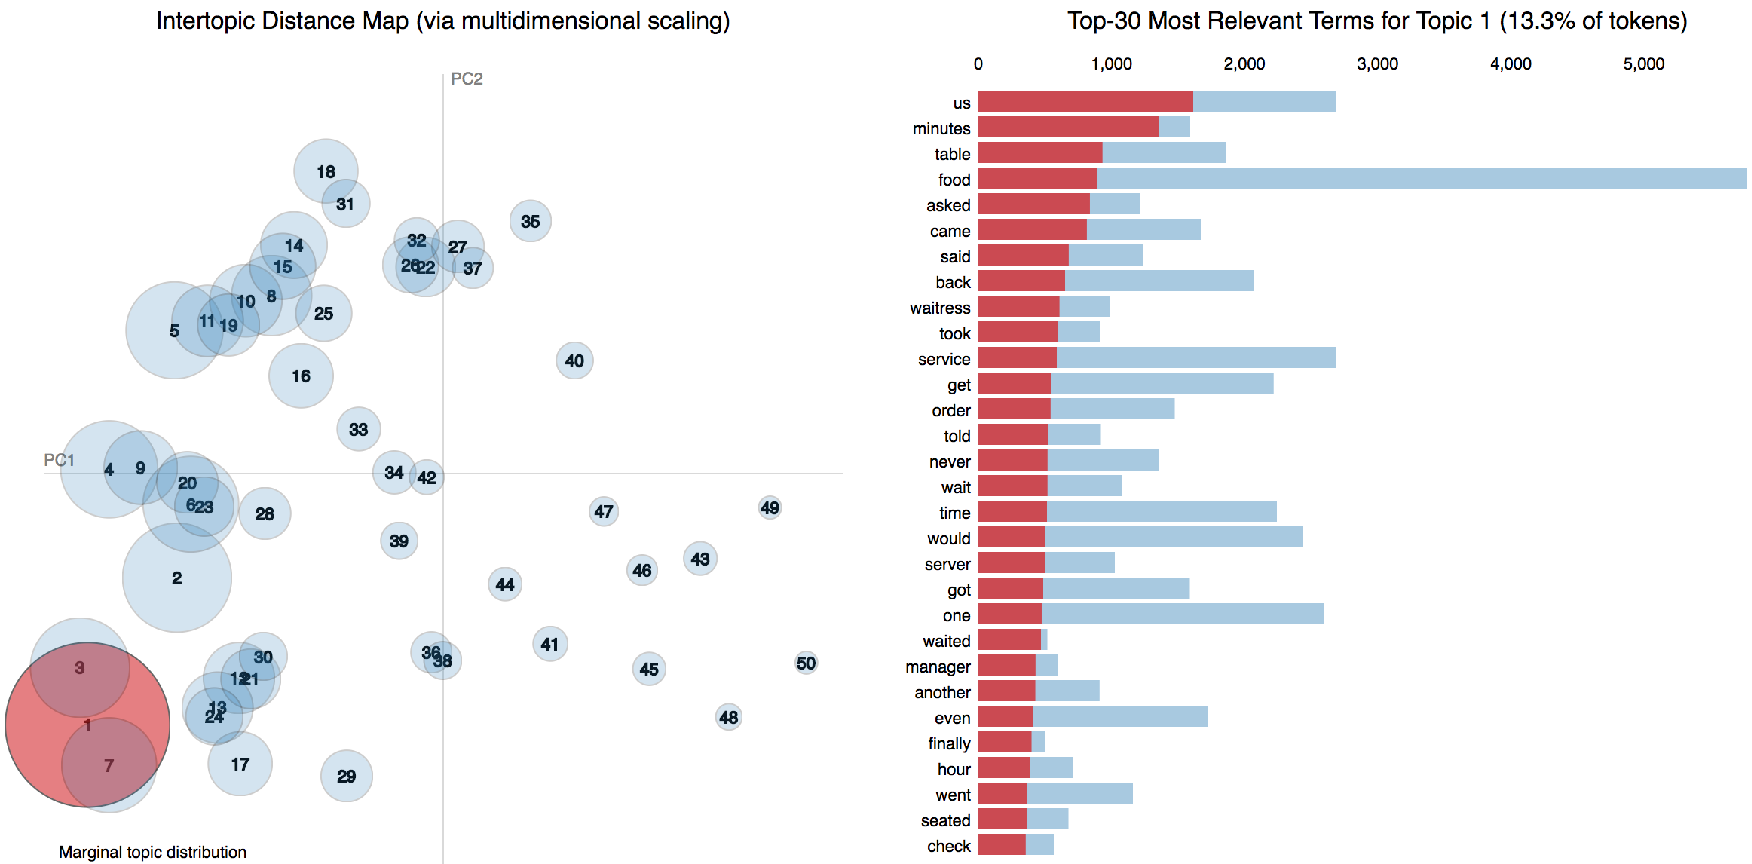
\includegraphics[width=0.5\linewidth]{second_image}
}
{
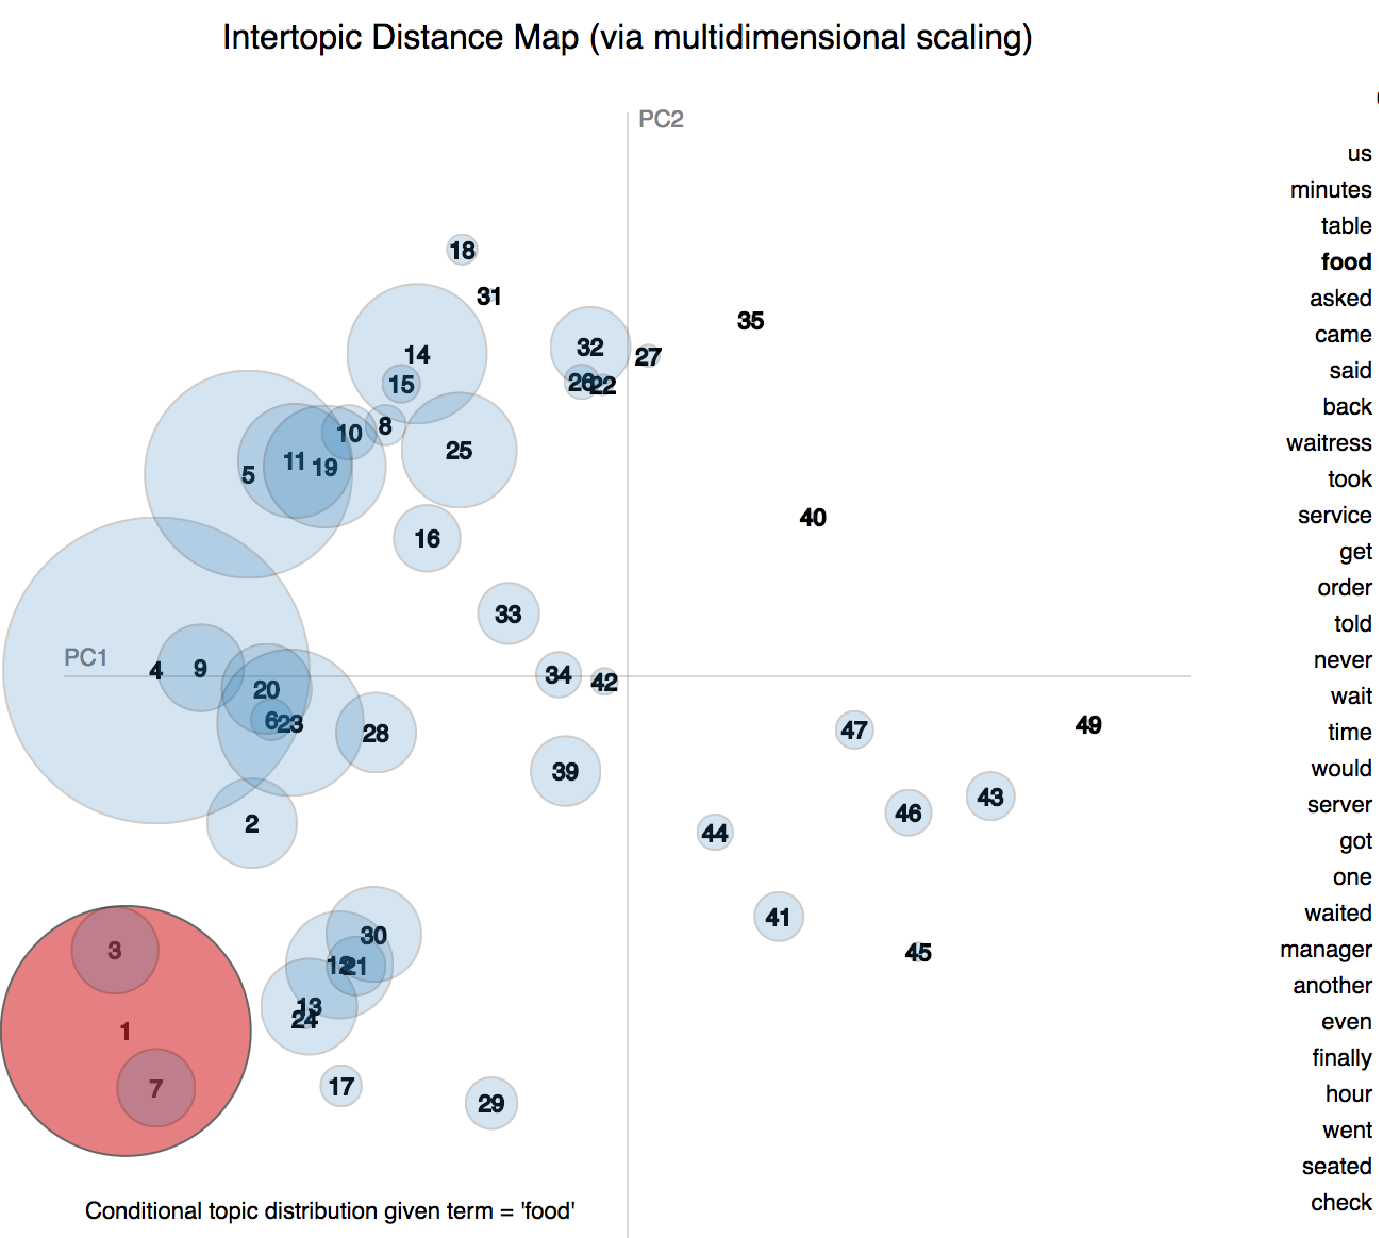
\includegraphics[width=0.3\linewidth]{third_image}
}
\end{figure}

Selecting a term on the right (as shown in the above image)  reveals the conditional distribution over topics (on the left) for the selected term (food). This kind of linked selection allows users to examine a large number of topic-term relationships in a compact manner.
To interpret a topic, one typically examines a ranked list of the most probable terms in that topic, using anywhere from 3 to 30 terms in the list. The problem with interpreting topics this way is that common terms in the corpus often appear near the top of such lists for multiple topics, making it hard to differentiate the meanings of these topics. So, ranking terms for a given topic in terms of both the frequency of the term under that topic as well as the term’s exclusivity to the topic, which accounts for the degree to which it appears in that particular topic to the exclusion of others. We call this relevance of a term to a topic that allows users to flexibly rank terms in order of usefulness for interpreting topics. Setting $\lambda = 1$ results in the familiar ranking of terms in decreasing order of their topic-specific probability, and setting $\lambda = 0$ ranks terms solely by their lift. We discovered how to set an optimal value of $\lambda = 0.6$ for topic interpretation from a case study.\\

Lets now see the most ranked words of topic 1 when $\lambda = 0, \lambda = 0.6$ and $\lambda = 1$.

\begin{figure}[h]
\centering
{
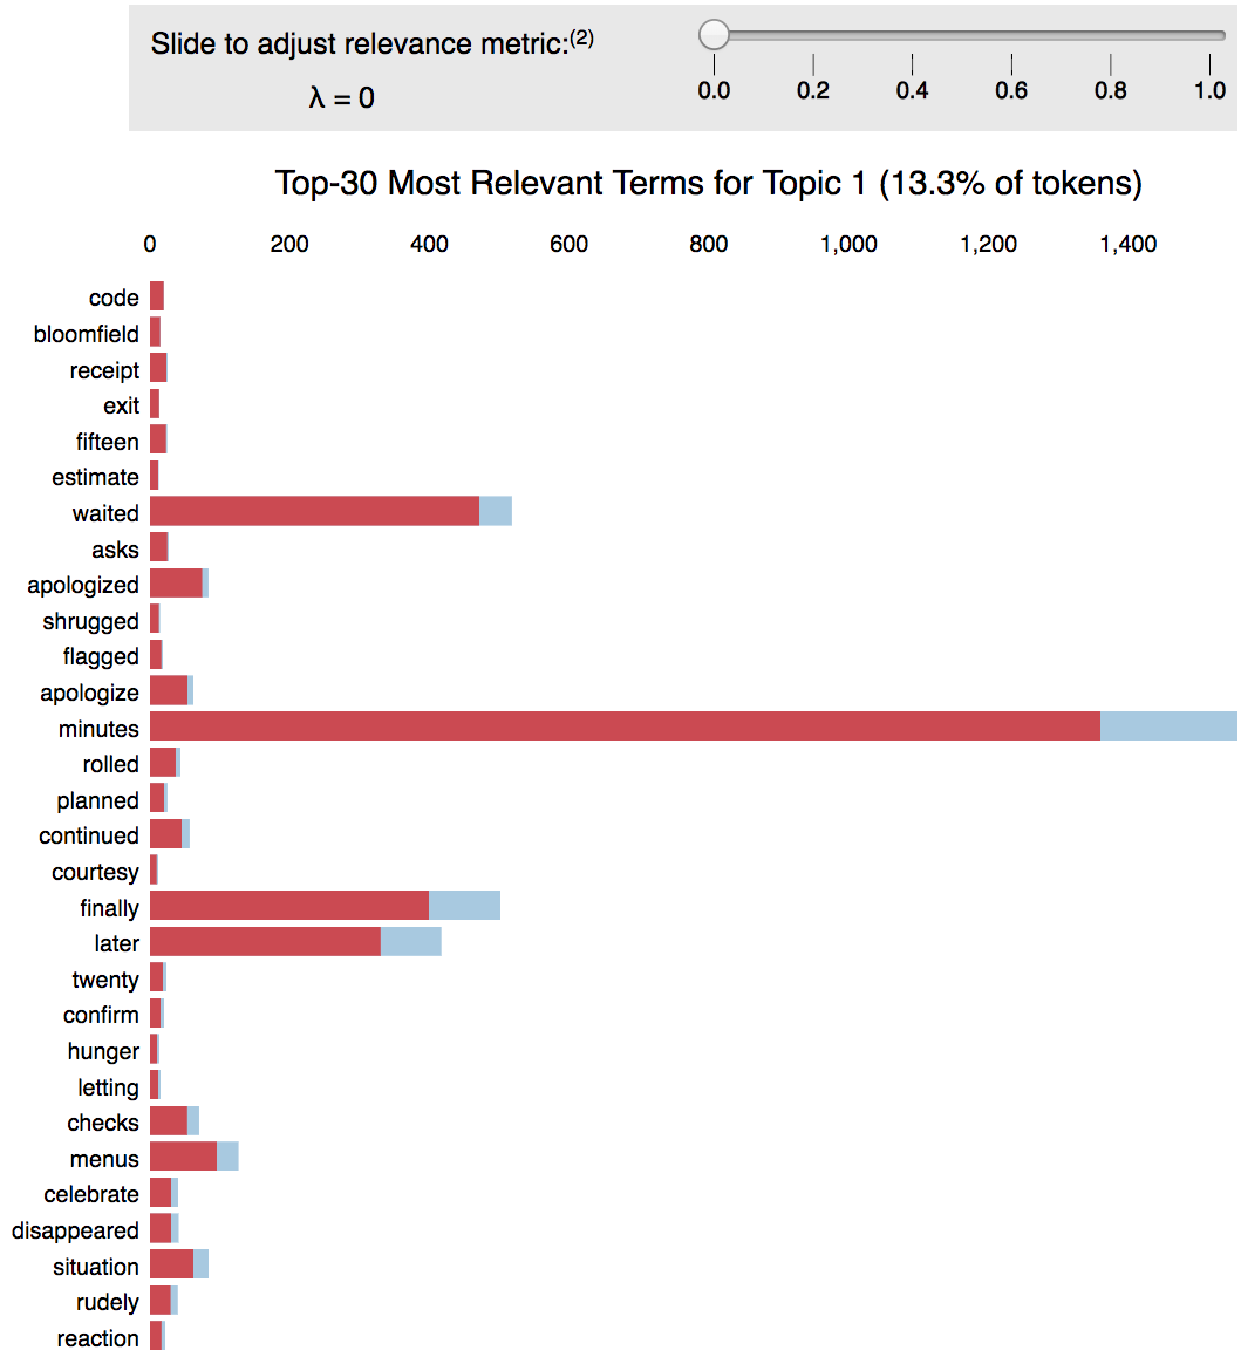
\includegraphics[width=0.3\linewidth]{lambda0}
}
{
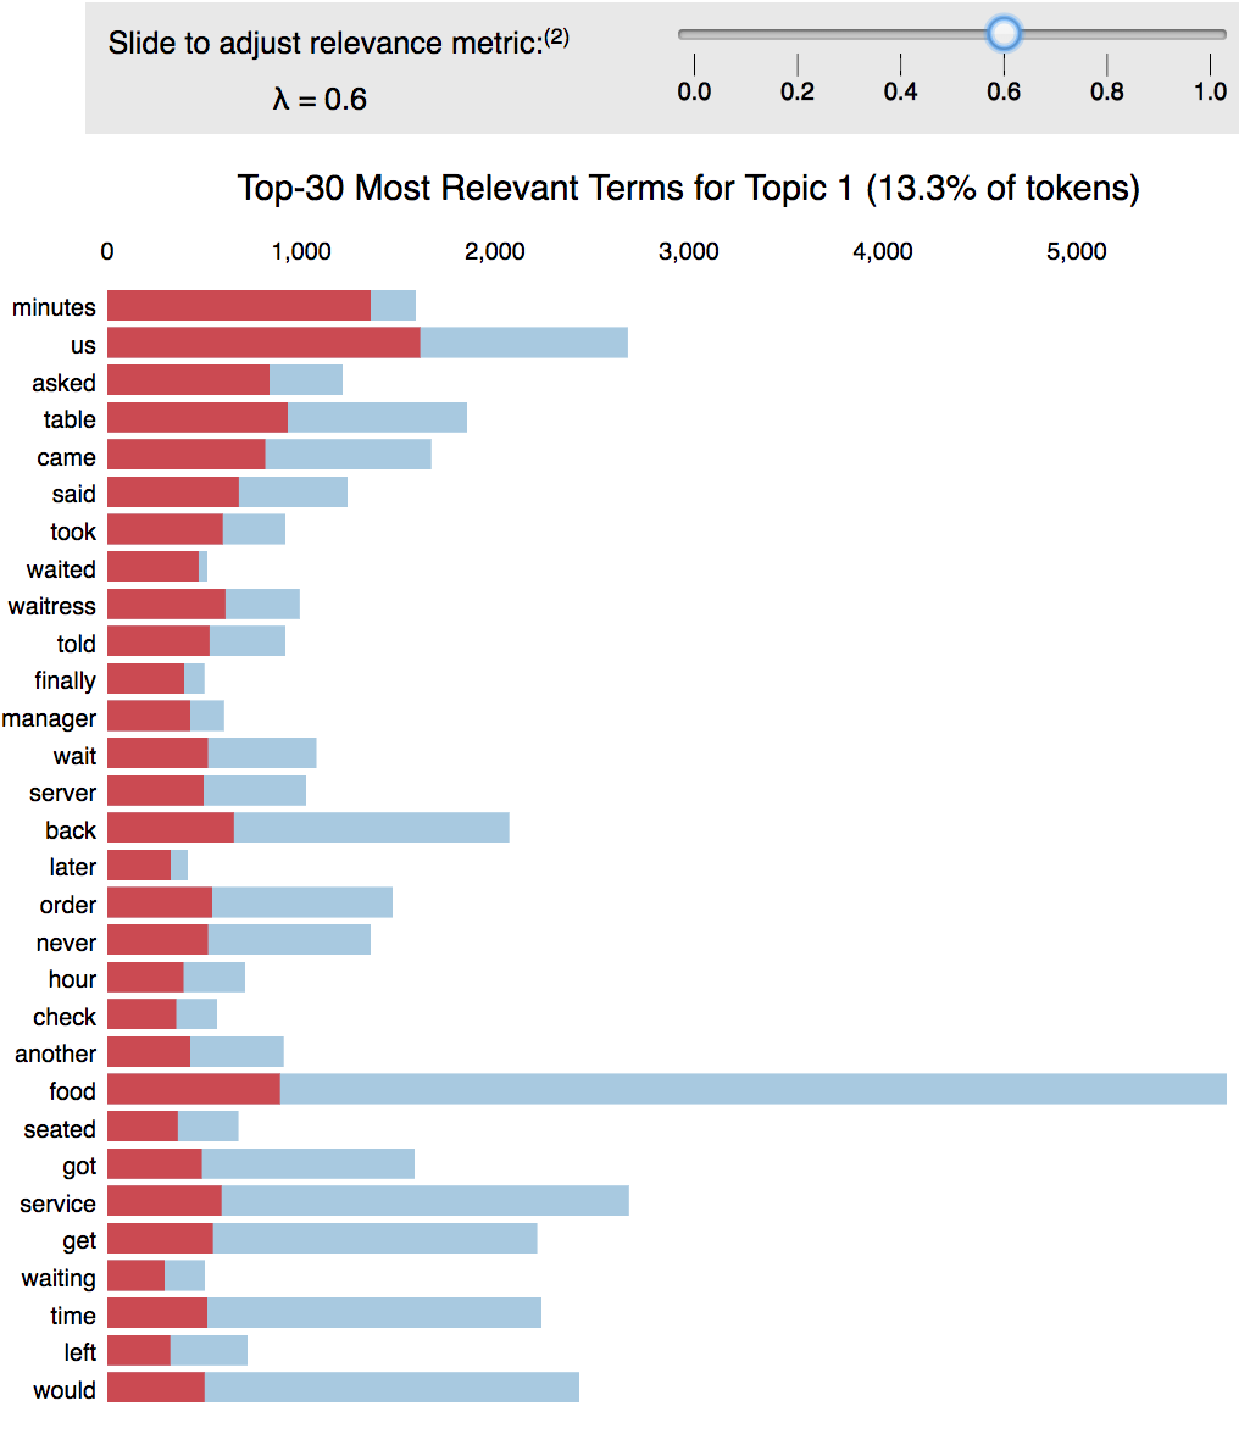
\includegraphics[width=0.3\linewidth]{lambda06}
}
{
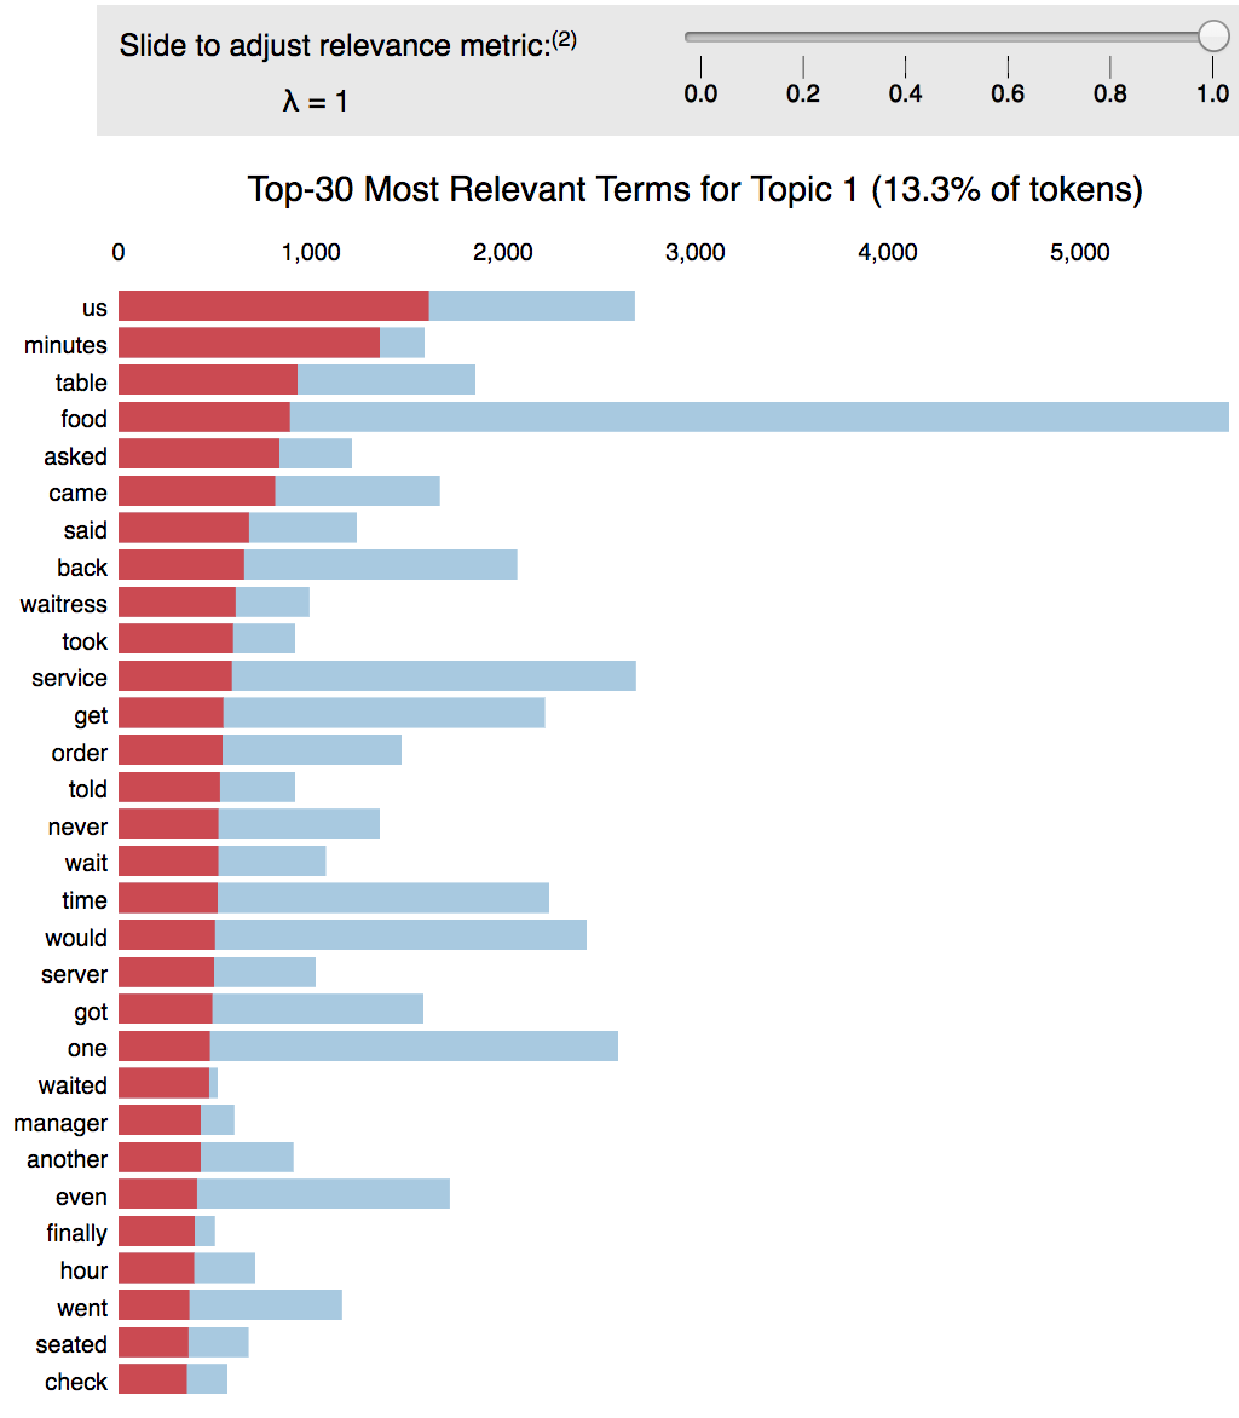
\includegraphics[width=0.3\linewidth]{lambda1}
}
\end{figure}

From the plots above, it can be clearly observed that when $\lambda = 0$, words that occur only this topic have a high ranking. When $\lambda = 1$, words that occur with highest number of times are ranked high, so we choose an optimum $\lambda = 0.6$ for better topic interpretation.\\

A similar kind of analysis can also be done with positive reviews. Download this\footnote{\url{https://github.com/emily-jean/yelp-data-mining/blob/master/project/topic-modeling/visualization_positive_50.html}} html page and run it in your browser for data exploration of the LDA model on positive reviews with 50 topics. Preivously, the number of topics chosen was an approximation. To get the optimal number of topics, Topic Coherence was used.\\

INSERT VYSHAAL'S UPDATE HERE	


\section*{4 Discussion}

Looking at the overall results of our data analysis and implementation, the group was pleasantly surprised by the
outcomes.\\
Although it seems that there is no strong relationship between type of cuisines and geographical neighborhood in Pittsburgh, there seems to be a more accurate clustering of areas based upon their attributes, such as upscale, divey, or casual. Our goal of auto-discovering neighborhoods did not come about in our results. In the future, we would like to run our implementation on varies cities, such as Las Vegas, to see if there are any differences on
cuisine and neighborhood connectivities among different cities.\\

ADD RECOMMENDATION SYSTEM DISCUSSION\\

ADD TOPIC MODELING DISCUSSION


\begin{thebibliography}{9}

\bibitem{datamining} 
Charu C. Aggarwal. 
\textit{Data Mining: The Textbook}. 
Springer 2015

\bibitem{massiveds} 
Jure Leskovec, Anand Rajaraman, Jeffrey D. Ullman. 
\textit{Mining of Massive Datasets}. 
Cambridge University Press, 2014

\bibitem{massiveds} 
Pang-Ning Tan, Michael Steinbach, Vipin Kumar. 
\textit{Introduction to Data Mining}. 
Pearson, 2005

\bibitem{massiveds} 
Xindong Wu, Vipin Kumar.
\textit{The Top Ten Algorithms in Data Mining}. 
Chapman and Hall, 2009

\bibitem{latexcompanion} 
Carson Sievert and Kenneth E. Shirley. 
\textit{LDAvis: A method for visualizing and interpreting topics}. 
https://nlp.stanford.edu/events/illvi2014/papers/sievert-illvi2014.pdf
 
\bibitem{topicmodeling}  
\textit{Topic Modeling}.
\textit{Machine Learning Summer School (MLSS), Cambridge 2009}. 
https://www.youtube.com/watch?v=DDq3OVp9dNA.

\bibitem{ldamodel}  
\textit{LDA Model}.
https://radimrehurek.com/gensim/models/ldamodel.html

\bibitem{sentiment}  
\textit{Method: documents.analyzeSentiment}.
\textit{Google Cloud Platform}. 
https://cloud.google.com/natural-language/docs/reference/rest/v1/documents/analyzeSentiment


\bibitem{stanford}  
\textit{Topic Modeling}.
[textit{Machine Learning Summer School (MLSS), Cambridge 2009}. 
https://nlp.stanford.edu/events/illvi2014/papers/sievert-illvi2014.pdf

\bibitem{amazon}  
\textit{Latent Dirichlet Allocation (LDA) with Python
}.
https://rstudio-pubs-static.s3.amazonaws.com/79360\_850b2a69980c4488b1db95987a24867a.html


\bibitem{gensim}  
\textit{News classification with topic models in gensim
}.
https://markroxor.github.io/gensim/static/notebooks/gensim\_
news\_classification.html

\end{thebibliography}



\appendix
\section{Appendices}
\subsection{GMM - Clustering of Neighborhood Cuisines in Pittsburgh}
\begin{figure}[h]
\centering
{
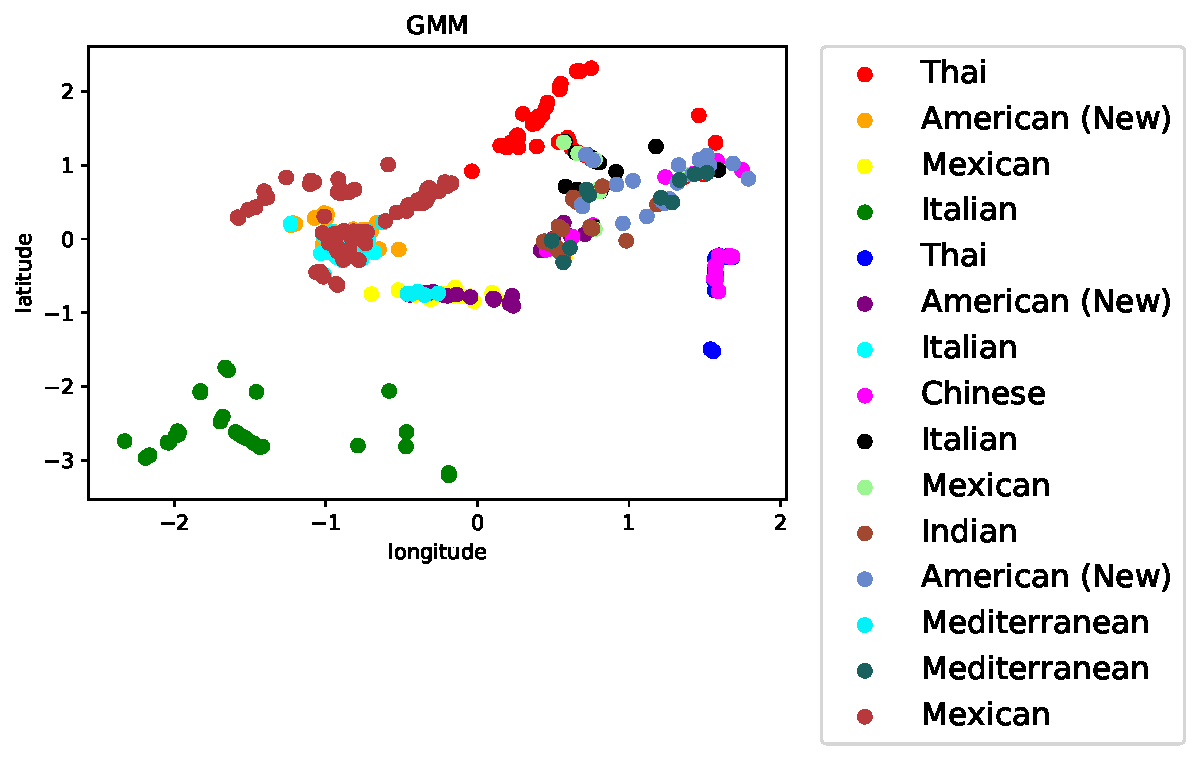
\includegraphics[width=0.5\linewidth]{gmm_cuisines}
}
\end{figure}

\subsection{LDA model on negative reviews with 50 topics}
\begin{figure}[h]
\centering
{
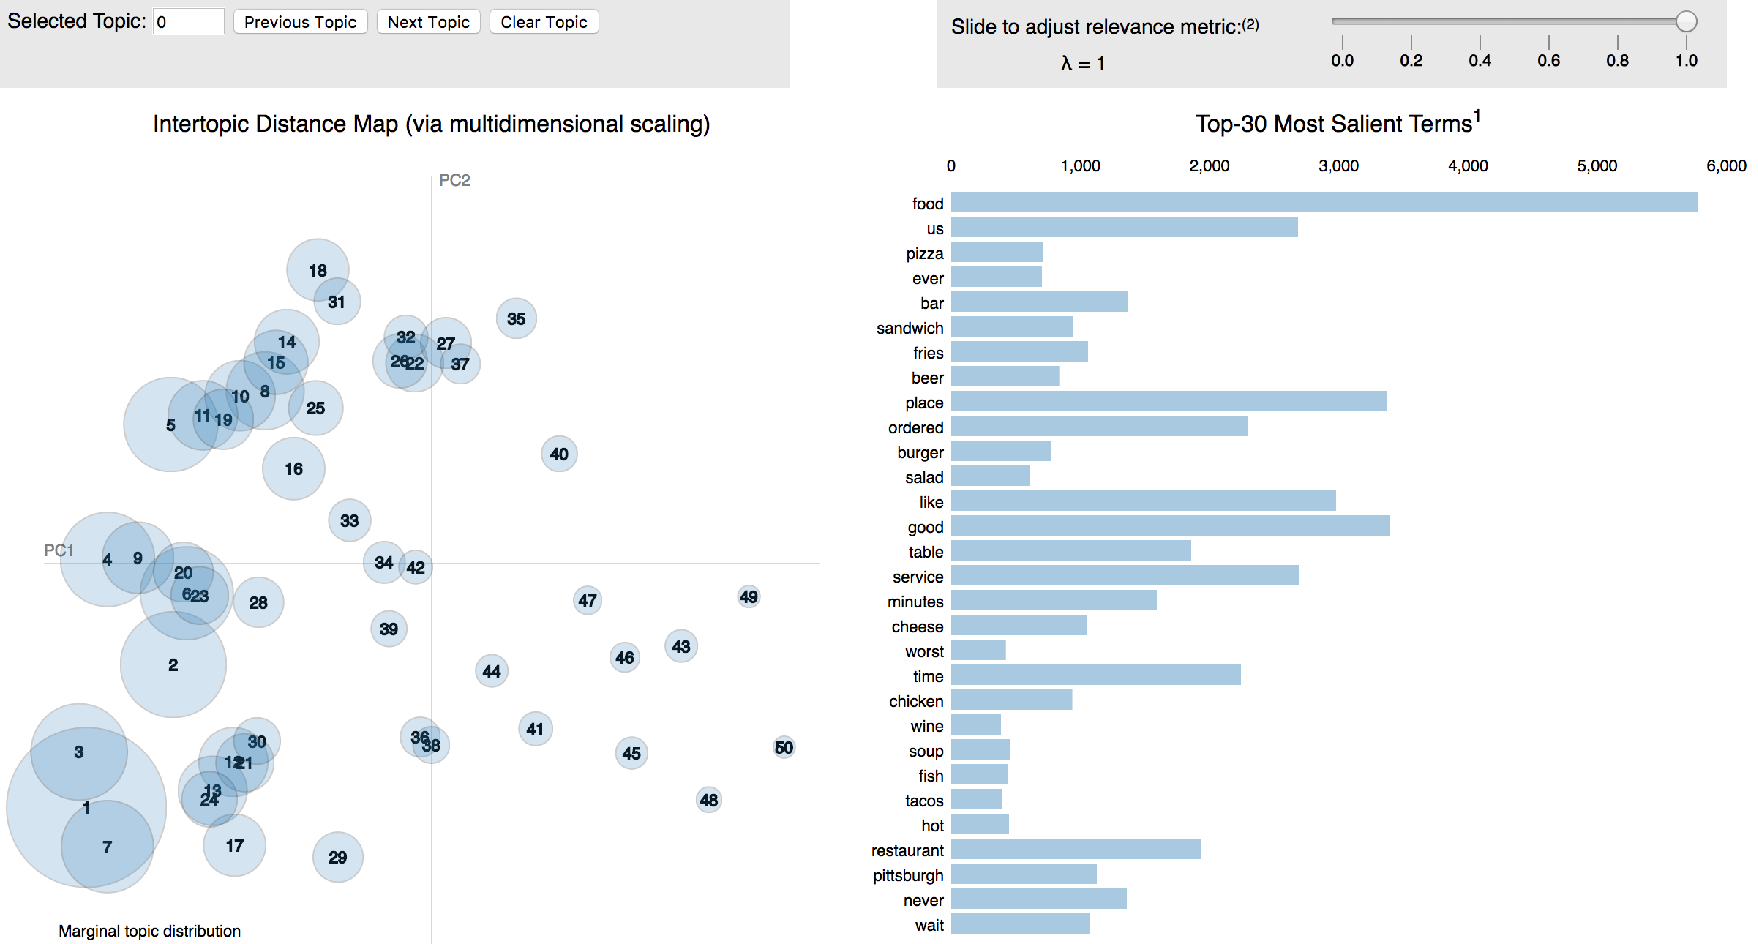
\includegraphics[width=0.6\linewidth]{first_image}
}
\end{figure}


\end{document}
